\documentclass[12pt,twoside]{reedthesis}
\usepackage{graphicx,latexsym} 
\usepackage{amssymb,amsthm,amsmath}
\usepackage{longtable,booktabs,setspace} 
\usepackage{eqnarray}
\usepackage{url}
\usepackage{underscore}
\usepackage{natbib}
\usepackage{verbatim}
\usepackage{algorithm}
\usepackage{algorithmic}
\newcommand{
\changefont}[3]{\fontfamily{#1}\fontseries{#2}\fontshape{#3}\selectfont}
%\newcommand{\procedure}[1]{{\changefont{pcr}{m}{n}\textbf{#1}}}
\newcommand{\procedure}[1]{{\tt#1}}
\newcommand{\var}[1]{{\mbox{\tt#1}}}
\newcommand{\im}[1]{{\em#1}}
%\newcommand{\var}[1]{#1}



\setlength{\parindent}{.5cm}
\title{Graph Algorithms on GPU Hardware}
\author{Ivan A. Malison}
\date{April 2012}
\division{Mathematics and Natural Sciences}
\advisor{James D. Fix}

\department{Mathematics}


\setlength{\parskip}{0pt}
\begin{document}

\maketitle
\frontmatter 
\pagestyle{empty}


%\chapter*{Acknowledgements}
  
%\chapter*{Preface}


\tableofcontents


\mainmatter 
\pagestyle{fancyplain}
\chapter*{Introduction}
\addcontentsline{toc}{chapter}{Introduction}
\chaptermark{Introduction}
\markboth{Introduction}{Introduction}

The Graphical Processing Unit is the first widely available parallel computer. Like most of the parallel computers that have been built, GPUs are basically SIMD....etc.

SIMD computers have largely been restricted to the solution of problems that are essentially data-parallel. The problems they solve practically beg to be solved in parallel fashion....etc.

The objective of this thesis is to explore the applicability of GPUs to problems that are data-parallel, but that the algorithms that are normally used to solve these problems do not, at first glance, lend themselves to the parallel processing afforded by GPUs. Specifically, we look at the Shortest Paths problem as it fits the aforementioned criteria, and it is a extremely important (and useful) and well studied problem in Computer Science.

\chapter{The Shortest Path Problem}



\section{Graphs Preliminaries}

A \im{graph} is a mathematical structure that comprises a set of objects and a set of connections between those objects. The members of the object set of a graph are called \im{vertices}, and the members of the connections set of a graph are called \im{edges}.

\begin{figure}[h!]
\begin{center}
\includegraphics{directedex.pdf}
\end{center}
\caption{A diagram depicting a directed graph of the ``hyperlinks to'' relation between Wikipedia articles.}
\end{figure}
Graphs come in two distinct flavors: \im{directed} and \im{undirected}. The edges of a directed graph are usually taken to represent a connection starting at some node and ending at another. If one imagines a graph as an object that allows travel between its vertices along its edges, a directed edge would represent a route that can only be traversed in one direction. This metaphor is useful in understanding the concept of a directed edge, but the reader should note that directed edges can also be used to represent other kinds of relationships. Strictly speaking, the characterizing feature of a directed edge is that it represents an asymmetric relationship between the vertices it connects.

As the reader has likely already ascertained, an undirected graph is one whose edges represent symmetrical relationships between the vertices they connect. If we return to the metaphor mentioned in the previous paragraph, an undirected edge would represent a route that can be traversed in both directions.

A directed graph might be useful in representing the hyperlink relationships between a group of Wikipedia articles. Each vertex in such a graph would represent a single Wikipedia article, and and edge $(u,v)$ would represent a hyperlink on page $u$ that leads to page $v$. An undirected graph cannot represent this structure because the existence of a link on page $u$ to page $v$ does not demand the existence of a link on page $v$ to page $u$.

Though an undirected graph can always be transformed into one that is directed (for each $\{u,v\}$ in the undirected graph $G_0$, add the edges $(u,v)$ and $(v,u)$ to the directed graph $G_1$ with the same vertex set), there are certain structures that are more accurately represented by an undirected graph. Take for example, a graph representing the geographic relationships between a group of countries, with each edge in the graph corresponding to a shared border between the countries represented by the vertices it connects. An undirected graph is appropriate in this situation because it allows each border to be represented by a single edge.

\begin{figure}[h!]
\begin{center}
\includegraphics[scale= .75]{SimpleGraph.pdf}
\end{center}
\caption{This figure will be the undirected graph country example in the final version.}
\end{figure}


A directed graph $G$ is a pair $(V,E)$, where $V$ is the vertex set of the graph,  and $E \subseteq V \times V \setminus \{(v,v) : v \in V\}$ where $\times$ refers to the cartesian product. The elements of the edge set of a directed graph are ordered pairs.

An undirected graph is a pair $(V,E)$, where $V$ is the vertex set of the graph and $E \subseteq \{ \{u,v\} : u,v \in V \}$. The elements of the edge set of an undirected graph are 2-subsets of $V$.

%Graphs by themselves are relatively uninteresting objects; It is possible to deduce certain general facts about graphs, like the number of different possible graphs on a certain number of vertices, but most of graph theory involves extending graphs by endowing them with additional structure. This paper involves two principle extensions that are described in the following paragraphs.

One natural graph structure to consider is a path. In informal terms, a path is a walk between the vertices of a graph along its edges. Though paths can be either finite or infinite, this paper restricts its inquiries to the domain of finite paths. There are a number of equivalent formal definitions of a finite path. One such definition follows:

A path $P$ in a graph $G = (V,E)$ is a sequence $(v_0, v_1, \cdots v_n)$ where each $v_i \in V$ and $(v_i, v_{i+1}) \in E$ for each consecutive pair of vertices in the Path.  Though this is the neatest definition of a path, the following equivalent definition is useful in later discussion:

In a directed graph, a path $P = (e_1, e_2, \ldots)$ has the property
 $$1 < i \implies e_i = (s_i, d_i), e_{i-1} = (s_{i-1}, d_{i-1}) \implies s_i = d_{i-1}$$

In an undirected graph, a  path $P = (e_1, e_2, \ldots)$ has the property
$$
1 < i, e_i = \{a_i, b_i\} \implies (a_i \in e_{i-1} \mbox{ and } b_i \in e_{i+1} ) \mbox{ or } 
(a_i \in e_{i+1} \mbox{ and } b_i \in e_{i-1} )
$$

In the case of an undirected graph, it may also be necessary to provide the starting vertex of the path.

The second graph extension that is essential to the topic of this paper is the concept of an edge weight function. An \im{edge weight function} of a graph $G = (V,E)$, assigns a real numerical value to each edge in the graph. A graph together with a weight function is called a weighted graph. Such graphs are typically given as a triple, $G = (V,E,f)$ where $V$ and $E$ are the vertex and edge sets of the graph, and $f : E \rightarrow \mathbb{R}$ is the weight function of the graph.

In a weighted graph, the path substructure introduced in the previous paragraphs can be naturally extended to have a weight. The weight of a path $P$ with edge sequence $\{e_i\}$ is given by

$$
\sum_i f(e_i)
$$

\section{Problem Description}

With these concepts in hand, it is now possible to describe the principal topic of this thesis, the \im{shortest path problem}. The shortest path problem takes place on a graph where vertices are taken to represent locations, edges are taken to represent direct routes between those locations, and edge weights are taken to represent the travel cost of each edge.

A natural application of this type of graph is to the problem of finding the shortest path between two locations on a roadmap. A graph used to represent this problem would have an edge for each atomic stretch of road over which there is no possibility of making a turn, and a vertex at any location where multiple routes can be selected such as an intersection.

The reader should resist the temptation to imagine that the locations, paths and distances in the shortest path problem must always be physical. The shortest path problem occurs in a wide variety of contexts including many where this is not the case. For example, in the problem of routing internet traffic a large distance value might represent high latency, or a lack of bandwidth between two virtual locations.

There are a number of variations of the shortest path problem. The road-map example described above is an example of the single-pair shortest path problem (because we are only interested in finding the shortest path from a particular place to another) where the weight function of the graph is always positive (because roads can't have negative length). Shortest path problems are classified by the kinds of shortest paths that need to be found, and the range of the edge weight function.

The terms used to classify these problems are:

\begin{itemize}
\item
The \im{single-pair shortest path} problem (SPSP) is the problem of finding the shortest path between two particular vertices in a graph
\item
The \im{single-source shortest paths} problem (SSSP) is the problem of finding the shortest paths to every vertex in the graph from a particular vertex.
\item The \im{single-destination shortest path} problem (SDSP) is the problem of finding the shortest paths from every vertex to a particular vertex.
\item The \im{all-pairs shortest paths problem} (APSP) is the problem of finding the shortest path between every pair of vertices in the graph (if it exists).
\end{itemize}

SPSP, SDSP can both be reduced to SSSP, and as such these three problems are usually studied as a group.

%\footnote{In the case of SPSP an SSSP algorithm is instructed to stop when the shortest path to the desired vertex is found. On an undirected graph, SSSP and SDSP are clearly the same. On a directed graph, SDSP is the same as SSSP with the orientation of each edge reversed; that is if $G_0 = (V, E_0, f)$, $E_1 = \{ (v,u) : (u,v) \in E_0\}$, $g((v,u)) = u,v$ and $G_1 = (V, E_1, f \circ g)$  the shortest path from $b$ to $a$ in $G_1$ is the shortest path from $a$ to $b$ in $G_0$. Thus SSSP on $G_1$ finds all the same shortest paths as SDSP on $G_0$.} APSP can also be solved in terms of SSSP, but there are also algorithms that specifically target APSP.
The shortest path problem has been studied extensively in the fields of mathematics and computer science. Efficient algorithms have been developed for every imaginable variation of the problem. The rest of this chapter describes some of the most notable of these algorithms.

\section{Graph Representation}

Graphs can be represented in a computer's memory in a variety of ways. The topic of graph representation will be discussed in detail in the later chapters of this paper. The remainder of this chapter employs a graph representation that consists of the following data types:

\setlength{\parindent}{0cm}

The \var{edge} data type has the following instance variables:

\begin{itemize}
\item \var{source} - the source vertex of the edge
\item \var{destination} - the destination vertex of the edge
\item \var{weight} - the edge weight assigned to this edge
\end{itemize}

The \var{vertex} data type has the following instance variables:

\begin{itemize}
\item \var{weight} - the path weight estimate
\item \var{predecessor} - the vertex that provided the current path weight estimate
\item \var{edges} - A list of edges for which the vertex is the source node.
\end{itemize}

\setlength{\parindent}{.5cm}

\section{The Bellman-Ford Algorithm}
\label{sec:bf}

The Bellman-Ford algorithm computes the single-source shortest paths of a weighted directed graph. It is notable both for its simplicity and the fact that it can be used on graphs with negative weights. We introduce some notation that will facilitate the description of this algorithm.
\vspace{1pc}

\setlength{\parindent}{0cm}
Let $G = (V,E,f)$ be a weighted, directed graph. Define the function $d_{u,v} : \mathbb{N} \rightarrow \mathbb{R}$ so that $d_{u,v}(n)$ is the weight of the shortest path from $u$ to $v$ that involves no more than $n$ edges. If no such path exists, $d_{u,v}(n) = \infty$.\footnote{We define $\infty + a = \infty$}
\setlength{\parindent}{.5cm}
\vspace{1pc}

Note that for $n \geq 0$:
\begin{equation}
\label{eq:did}
d_{u,v}(n+1) = \min \{d_{u,w}(n) + f(w,v) : w \in V, \, (w,v) \in E \} \cup \{d_{u,v}(n)\}
\end{equation}
This identity implies that the shortest paths of length $n+1$ from a source $s$ can be computed if every shortest path of length $n$ starting at $s$ is known. This insight informs the design of the Bellman-Ford algorithm. 

The Bellman-Ford algorithm does not perform the minimization in this identity directly. Instead, it performs a relatively simple procedure called \procedure{edge-relax}, over the edges of the problem graph. An edge-relax of $(u,v)$ updates the shortest path weight value at $v$ to be the weight estimate at $u$ added to the edge weight of $(u,v)$, provided that this value is smaller than the current path weight estimate at $v$. Pseudo-code for this procedure is provided below:

\begin{algorithm}[h!]
\caption{edge-relax(edge)}
\label{edgerelax}
\begin{algorithmic}
\IF{edge.destination.weight $>$ edge.source.weight + edge.weight}
\STATE edge.destination.weight = edge.source.weight + edge.weight
\STATE edge.destination.predecessor = edge.source
\ENDIF
\end{algorithmic}
\end{algorithm}

\vspace{1pc}

If the weight value of each vertex $w$ is $d_{u,w}(n_{w1})$, where $n_w > n$, it can be concluded that after every edge in the graph is relaxed once, the weight value of each vertex will be $d_{u,w}(n_{w2})$ where $n_{w2} > n$. What this admittedly convoluted statement is saying is:

\begin{quote}
If we have the shortest path of length less than $n$ {\em or better} (i.e. allowing smaller path weights, but possibly with more edges) at each vertex, we will have the shortest path length of $n+1$  {\em or better} after all edges are relaxed.
\end{quote}

It is easy to see that this is true. Let $P_{s,w}$ be a shortest path of length smaller than $n+1$ to $w$, whose penultimate vertex is $xw_{0}$. The subpath of $P_{s,w}$ ending at $w_{0}$, must be the shortest path from $s$ to $w_0$ of length $n$; if not $P_{s,w}$ would not be the shortest path of length $n+1$ to $w$. Since every vertex contains the weight of the shortest path to that vertex of with at least $n$, either $w_{0}$ has the weight of this subpath or it has a smaller weight that comes from a path with more edges. This means that when the edge $(w_0, w)$ is relaxed, either the path $P_{s,w}$ is considered, or the a longer path with smaller weight is considered.

The reason the ``or better'' portion of this statement is necessary is that a series of edge-relaxes that occur one after another could produce multiple extensions to the same path. If we imagine that the shortest path of length 2 from $s$ to $v$ consists of the edges $(s,b)$, $(b,v)$, a single set of edge relaxes where $(s,b)$ is relaxed before $(b,v)$ will update the weight value of $v$ to be the weight of this path.
\vspace{1pc}

Bellman-Ford relies on the fact that the shortest paths of length 0 can be determined a priori. Specifically, $d_{u,v}(0) = 0$ if $u = v$ and $d_{u,v}(0) = \infty$,  if $u \neq v$. This means that shortest paths of length $n$ can be obtained by initializing each vertex to have its shortest path weight from the source vertex of length 0, and running $n$ sets of edge relaxes. To obtain the unconstrained shortest paths of the graph, only $|V|-1$ sets of edge relaxes need to be performed. This is because a shortest path in a graph with $|V|$ vertices can not traverse more than $|V|-1$ edges. Any path that traverses more edges visits more than $|V|$ vertices, which means that (by the pigeonhole principle) it would have to visit some vertex twice. In other words, some portion of the path would start and end at the same place. A path with a cycle is only shorter than the same path where the cycle is cut out if the cycle has negative weight. In that case, a shorter path can be obtained by traversing the cycle more than once before continuing the rest of the path. This is all to say that when there is a negative cycle available between two vertices in a graph, there is no shortest path between them. A path with arbitrarily small weight can be obtained by traversing the cycle enough times.

The Bellman-Ford algorithm performs $|V| - 1$ sets of $|E|$ edge-relaxes, or $(|V| - 1)\cdot E$ total edge-relaxes. Since each edge-relax can be performed in constant time, the runtime of the algorithm is $\mathcal{O}(|V||E|)$. Bellman-Ford is the fastest known algorithm for computing shortest paths on graphs with negative edge weights, but for graphs with non-negative edge weighs, there are faster methods.

\section{Dijkstra's Algorithm}

Dijkstra's algorithm solves the SSSP problem on a weighted directed graph with arbitrary non-negative edge weights. Like the Bellman-Ford Algorithm, it provides the solution in the form of a path tree that is rooted at the source vertex. Before we present the algorithm in detail, we present several preliminaries to facilitate the explanation of the algorithm.

\subsection{Preliminaries}

\setlength{\parindent}{0cm}
Let $G = (V,E)$ be a directed graph, and let $f : E \rightarrow \mathbb{R^+}$ be a weight function for $G$. Furthermore, let $s \in V$ and let $S \subset V$ be a set of vertices (containing $s$) for which the correct shortest paths from $s$ to each vertex $u \in S$ and their respective weights are known. Define $d : S \rightarrow \mathbb{R^+}$ to be the function that provides the weight of the shortest path from $s$ to its argument and define $e : V \setminus S \rightarrow \mathbb{R^+}$ as

$$
e(u) = \min \{ f(v,u) + d(v) \, | \, v \in S, \; (v,u) \in E \}
$$

We set $e(u) = \infty$ if there is no qualifying $v \in S$.


%%Note that though there may be more than one $v$ that minimizes $f((v,u)) + d(v)$.

Since $V$ is a finite set, there is some $a \in V \setminus S$ such that for every $u \in V \setminus S$, $e(a) \leq e(u)$.
\vspace{1pc}

\textbf{Claim:} $e(a)$ is the weight of any shortest path from $s$ to $a$.

\begin{proof}
Suppose that $e(a)$ is not the weight of the shortest path(s) to $a$. Then $\exists$ a path $P =(s, v_1, v_2, \ldots a)$ of $G$ starting at $s$ and ending at $a$ such that $w(P) < e(a)$. Since $P$ starts at $s$ which is in $S$, and ends at $a$ which is not in $S$, there is a first vertex that is not an element of $S$ that appears in the path $P$. Let $c$ be the first such vertex appearing in $P$, and let $b$ be the vertex in $P$ that precedes this vertex. We set $P_{s,b}$ to be the portion of $P$ starting at $s$ and ending at $b$, and $P_{c,a}$ to be the portion of the path starting at $c$ and ending at $a$.
\vspace{.5pc}

Because $c \in V \setminus S$, we know that $e(a) \leq e(c)$. Since $b \in S$ and $(b,c) \in E$ (since it appears in $P$), we know that $e(c) \leq d(b) + (b,c)$. Because $P_{s,b}$ is a path from $s$ to $b$, we know that $d(b) \leq w(P_{s,b})$, since $d(b)$ is the shortest any path to $b$ from $s$ can be. Combining all of this we get

\begin{equation}
e(a) \leq e(c) \leq d(b) + f((b,c)) \leq w(P_{s,b}) + f((b,c))
\label{eoc}
\end{equation}  

We express the weight of the path $P$ in terms of $P_{s,b}$ and $P_{c,a}$. 

\begin{equation}
w(P_{s,b}) + f((b,c)) + w(P_{c,a}) = w(P) < e(a)
\label{pweight}
\end{equation}

Because $f$ is a non-negative function, every path in $G$ has non-negative weight. Thus:

\begin{equation}
w(P_{s,b}) + f((b,c))  \leq w(P_{s,b}) + f((b,c)) + w(P_{c,a})
\label{worest}
\end{equation}

Combining equations \ref{eoc}, \ref{pweight} and \ref{worest} we get

$$
e(a) \leq e(c) \leq w(P_{s,b}) + f((b,c))  \leq w(P) < e(a)
$$

which is clearly a contradiction. We conclude that $e(a)$ must in fact be the weight of any shortest path from $s$ to $a$.
\end{proof}

\setlength{\parindent}{.5cm}

The proof above tells us that in a graph with positive edge weights, a subset of vertices whose shortest paths are known can always be extended with the addition of the vertex not yet in the set whose distance from the vertices currently in the set is smallest. The idea behind Dijkstra's algorithm is to do this repeatedly, until every vertex in the graph is in the set of vertices with known shortest paths.

Dijkstra's algorithm implements this process with a construct called a \im{priority queue}. Like a stack or a FIFO queue, a priority queue is a storage data type with a callable method that automatically selects and dequeues one of its stored element according to a predetermined procedure. Data elements are inserted into a priority queue together with a numerical value that allows them to be ranked amongst the other values that have been inserted into the queue. A priority queue uses the priority value of its elements to determine which one should be dequeued next. A min priority queue --a priority queue that always dequeues the element with the smallest priority value-- implements the following procedures:

\begin{itemize}

\item \procedure{insert(value,key)} - inserts the element \var{value}, with priority \var{key}.

\item \procedure{dequeueMin()} - returns the element with the smallest priority that is currently stored in the \im{priority queue}, and removes it from the queue.

\end{itemize}

\subsection{Algorithm Description}

Dijkstra's Algorithm begins in much the same way as the Bellman-Ford algorithm; the path-weight value of the source vertex is set to be 0, and the path-weight value of every other vertex in the problem graph is set to be positive infinity. The value of the the shortest-path from the source vertex $s$ to itself is known a priori --- it is the trivial path of length and weight 0. Thus the set $S$ from the proof in the previous section is initialized to be the singleton set containing the source vertex $s$.

The min priority queue that we described earlier is used to manage the set of vertices whose shortest paths are not yet known. Throughout the algorithm, each vertex in the priority queue has a priority that corresponds to the shortest path to that vertex that only passes though elements in $S$ before reaching that vertex (this value is set to positive infinity if no such path is exists). That is, the priority value of a vertex $u$ in the priority queue is exactly $e(u)$. Provided that this property holds true, the dequeueMin() function will always provide a vertex whose shortest path estimate can be finalized.

As the min priority queue handles the vertex selection process entirely by itself, maintaing the appropriate priority values for each vertex constitutes most of the work of Dijkstra's algorithm. When a vertex is dequeued from the priority queue (i.e. added to the set $S$), it is likely that the priority values of some of the vertices will no longer be accurate. However, not every vertex in the graph needs to be examined. The function $e$ only takes on the values of shortest paths where the final edge in the path starts at a vertex in $S$ and ends at a vertex not in $S$. No shortest path to a vertex in $S$ will pass through the newest addition to the set, so the only vertices whose new shortest paths must all reach their destination over an edge from the newly added element. That is, only vertices $v$ for which $(a,v) \in E$ where $a$ is the newly added vertex need to be updated.

\subsection{Pseudo-Code and Analysis}

In the pseudo-code that follows, the variable \var{vertices} is a reference to a list object that contains all of the vertices in the problem graph, the variable \var{queue} is the min priority queue that is used to store the vertices in the graph, and the edge and vertex data types are defined as they were in the Bellman-Ford section. 

\begin{algorithm}[h!]
\caption{Dijkstra's Algorithm}
\label{dijkstrapseudo}
\begin{algorithmic}[1]
\FOR{vertex $\in$ vertices, vertex $\neq$ source}
\STATE vertex.weight = $\infty$
\STATE queue.insert(vertex, vertex.weight)
\ENDFOR
\STATE source.weight = 0
\STATE added = source
\WHILE{added is not null}
\FOR{edge $\in$ added.edges}
\STATE relax = edge.source.weight + edge.weight
\IF{relax $<$ edge.destination.weight}
\STATE edge.destination.weight = relax
\STATE edge.destination.predecessor = edge.source
\STATE queue.setpriority(edge.destination, relax)
\ENDIF
\ENDFOR
\STATE added = queue.dequeueMin()
\ENDWHILE
\end{algorithmic}
\end{algorithm}

We begin our analysis of Dijkstra's algorithm by noting that the above pseudo-code contains three non-atomic operations. The calls \procedure{queue.insert} on line 3, \procedure{queue.setPrirority} on line 13 and \procedure{queue.dequeueMin} on line 16 initiate the execution of procedures that cannot be assumed to execute in constant time. The obvious question is ``How long do each of these procedures take?''

The answer is somewhat complicated. The concept of a priority queue does not refer to any particular kind of data structure or procedure; rather, it is a protocol that describes a set of behaviors without specifying their implementations. There are a number of ways that one can implement a priority queue, and the runtime of each queue operation varies depending on which implementation is used. A full discussion of priority queue implementation would not be relevant to the topic of this paper; a thorough treatment of the topic can be found in nearly any undergraduate algorithms text book.

Because Dijkstra's algorithm makes extensive use of its min priority queue, it is impossible to make any meaningful statements about its runtime without reference to the runtime of each queue operation. We use the functions $i(\cdot)$, $s(\cdot)$ and $d(\cdot)$ to stand in for the runtimes of the insert, setPriority and dequeue operations respectively. Once the analysis of the algorithm is finished, we will cite the asymptotic runtimes of these functions in a number of priority queue implementations, and apply any possible further reductions that these values enable.

When it is executed on a graph with $n$ vertices and $m$ edges, the body of the main loop of Dijkstra's algorithm (which starts on line 7 in the above pseudo-code) is executed exactly $n$ times. This is because every iteration of the loop corresponds to the addition of a vertex to the set of vertices with known shortest paths. Though the for loop on line is 8 is inside the main loop, its analysis is conducted separately; the body of that loop is executed exactly $m$ times because every edge has exactly one starting vertex, and the loop is executed over the edges of each vertex exactly once. Thus the only operation we need to account for in the main loop is the queue.dequeue operation on line 16. Thus the worst case running time of the main loop is $\mathcal{O}(n\cdot d(n))$.

All of the operations that take place in the body of the for loop starting line 8 except for queue.setpriority execute in constant time. Since this loop executes exactly $m$ times, the worst case total for this loop is $\mathcal{O}(m \cdot s(v))$.

The queue initialization loop starting on line is obviously executed $\theta(n)$ times. Thus the worst case runtime of this loop is $\mathcal{O}(n \cdot i(n))$. 

Adding the values found in the last three paragraphs, gives the upper bound for the worst-case runtime of Dijkstra's algorithm $\mathcal{O}(n(i(n) + d(n)) + m(s(n))$.

\vspace{1pc}

One way to implement a priority queue is to use an array to store inserted values. If the number of values that will be inserted into the queue is known ahead of time, as in the case of Dijkstra's algorithm, the priority queue functions can be implemented quite easily. The insertion function takes place in constant time, and merely requires a counter pointing to the next empty slot. With this priority queue implementation, there is no need to store the priority and weight values of a vertex separately, so the queue.setpriority operation is simply an assignment to the value vertex.weight, which occurs in constant time. The array stores no information about the relative priorities of the inserted vertices, so the dequeueMin operation requires a linear search of the inserted values. The worst case runtime of linear search on $n$ objects is $n$. With this implementation of a priority queue, the worst case runtime of Dijkstra's algorithm is given by

$$
\mathcal{O}(n(i(n) + d(n)) + m(s(n)) = \mathcal{O}(n(1+n) + m(1)) = \mathcal{O}(n^2 + m)
$$

Since a directed graph has no more than $n(n-1)$ edges, $\mathcal{O}(n^2 + m) \subseteq \mathcal{O}(n^2 + n(n-1) = \mathcal{O}(2n^2) = \mathcal{O}(n^2)$.

\vspace{1pc}

This bound on the runtime of Dijkstra's algorithm can be improved by implementing the min priority queue with a more sophisticated data structure called a Fibonacci heap. A detailed explanation of this priority queue implementation is beyond the scope of this paper, so we simply note that this implementation can be shown to have amortized costs of $\mathcal{O}(\log n)$, $\mathcal{O}(1)$ and $\mathcal{O}(1)$ for its \var{dequeueMin}, \var{insertion} and \var{setPriority} operations respectively. This gives a runtime bound of 

$$
\mathcal{O}(n(1+ \log n) + m(1)) = \mathcal{O}(n(\log n) + m)
$$

Technically speaking, this is only an improvement given that the number of edges in the graph is $o(n^2/\log n)$. Executing a Fibonnaci-Heap implementation of Dijkstra's algorithm on a graph with $m = \mathcal{O}(n^2)$ edges yields a runtime of $\mathcal{O}(n^2)$.

\chapter{GPU Hardware}

The following chapter describes the basic design of modern GPUs and the factors that informed these design decisions.
%%Though the architectural features highlighted in this section will inform the development of algorithms developed later in the paper, keep in mind that this description is a something of a cartoon, and that actual GPU hardware is usually more sophisticated.

\section{The Graphics Pipeline}

To this day, the design of GPU architecture has been primarily aimed at the process of rendering three dimensional graphics. Though this process is only tangentially related to the topic of this paper, it is impossible to present the topic of GPU hardware without a brief discussion of the specific type of computation at which it is primarily aimed.

The process by which GPUs render graphics is called the \im{graphics pipeline}. Though the details of the graphics pipeline are constantly evolving, the basic stages of the procedure have remained the same. What follows is a rough outline of the major stages of the graphics pipeline.

\subsection{Overview}

The input to the graphics pipeline consists of an array of polygons --usually triangles-- that are positioned in a three dimensional coordinate system. These polygons describe the facets that constitute the surfaces of objects in a model of a 3-D scene. The ultimate goal of the graphics pipeline is to take this data, together with lighting and texture data, and render it as a 2D image that can be displayed on a screen.

\begin{figure}[h]
\begin{center}
\includegraphics{graphicspipeline.pdf}
\end{center}
\caption{The graphics pipeline.}
\end{figure}
\vspace{1pc}

The process begins with a per vertex operation stage, where basic arithmetic is applied to each vertex that makes up one of the triangles in the input array. The vertices are shaded according to their interactions with light in the scene, and sometimes they are rotated and translated. Then the vertices are mapped on to screen space according to some reference frame that is often called the virtual camera.  At this point the vertices are reassembled into new primitives, and vertices that will not appear in the final image are discarded.

The next major stage is the \im{rasterization} phase. This phase calculates which pixels in the final image will be covered by each primitive from the previous phase. Each primitive generates what is called a \im{fragment} at every pixel location that it covers. In the rest of the graphics pipeline, operations take place on a per fragment basis. Note that there is not necessarily a one-to-one association between fragments and pixels because it is possible for multiple primitives to cover the same pixel.

The fragment stage computes a final color value for each fragment generated in the rasterization phase. This is done by combining color information from vertices and light sources. It is during this phase that images known as textures are mapped on to the surface of polygons.

The final stage computes the final color value for each pixel, usually by selecting the fragment value that is closest to the camera. The final pixel colors are written to a special location in GPU called the frame buffer, from which images can be quickly and easily displayed.

\subsection{The GPU Approach}

The distinguishing feature of the graphics pipeline is its enormous potential for parallelism. Within each stage, the operations that are performed on the primitive data elements of that stage can be performed completely independent of one another. Furthermore, operations can be performed on primitives that have reached one stage of the graphics pipeline even if not all of the primitives have yet reached that stage of the pipeline.

If one were to implement the graphics pipeline on a sequential computer they would be forced to start at some stage with some element (or group of elements), and walk through the entire graphics pipeline with that element and its descendants. Then the CPU would move on to the next group of elements, again performing each stage separately. The CPU divides the graphics pipeline in time; at any given moment, it is devoting all its resources to performing the operations at a particular stage for a particular element.

The GPU takes an entirely different approach to implementing the graphics pipeline. Instead of performing each stage of the graphics pipeline at a different point in time, it divides its resources amongst the different stages of the graphics pipeline, and performs them all at the same time. This approach to the problem of graphics rendering has proved to be highly successful for a variety of reasons. The most important of these is that dividing the problem in this manner allowed the hardware that is working in each stage to exploit the data parallelism at that stage. Instead of operating on a single element at a time, a component in the graphics pipeline works on a huge number of objects at a time. Though a graphics component may take quite a long time to compute the desired values for any particular element, it compensates for this by having enormous throughput. Because the different stages of the graphics pipeline exhibit parallelism over different kinds of primitives, this would not be possible if GPUs attacked the pipeline as a whole. Since each primitive element undergoes the same set of operations at each stage, this parallelism is accomplished without complicated control circuitry governing the execution on each element.

\subsection{The Evolution of GPU Architecture}

Another reason for the initial success of the GPU approach was that many of the computations in the graphics pipeline could be performed more efficiently with specialized hardware. The early graphics hardware architecture, now generally referred to as the fixed-function graphics pipeline, used specialized non-programmable circuitry for each stage in the graphics pipeline. But this design paradigm was not without its downsides. For example, while programmers could control things like the position and intensity of lighting sources through the graphics APIs that controlled these early GPUs, they could not control the algorithm that computed the interactions of those lighting sources with vertices and primitives.

This meant hardware vendors had to add entirely new circuitry to implement any new features that developers requested. For certain kinds of complex lighting and shading effects, it was entirely unfeasible to design circuitry with only those functions in mind. This led graphics hardware vendors to design GPUs where the per vertex operations of the graphics pipeline were performed by hardware that could be directly programmed by application developers. This evolution in graphics hardware proved to be very successful, and eventually, the per fragment stage of the graphics pipeline also became programmable.

Initially, the various programmable stages of the graphics pipeline featured different instruction sets that were suited to the roles they performed. But as the per vertex and per fragment programs that developers were building became increasingly complex, the needs at each stage converged. This led graphics hardware vendors to develop the unified shader model, an architecture paradigm where all of the programmable stages of the graphics pipeline are performed on a single array of multiprocessors. This revolution in graphics card architecture was important for two major reasons.

The first of these was that it allowed GPUs to load balance the stages of the graphics pipeline. A fixed-function graphics pipeline was only as fast as its slowest component, because if one stage of the graphics pipeline required more time than the others, all of the other components would become inactive while the slower component finished its computation. With the unified shader model, the resources of the graphics card could be dynamically allocated between the various programmable stages of the graphics pipeline, and most of the hardware would remain active throughout the entire computation.

The other major advantage of the unified shader model has nothing to do with the graphics pipeline. With the unified shader model, the instruction sets of the multiprocessor arrays of GPUs have come to resemble those of general purpose processors. This combined with the release of APIs like CUDA and OpenCL that allow programmers to bypass the graphics pipeline and directly access the multiprocessor arrays of GPUs has greatly facilitated the practice of GPU computing.

\section{The Architecture of the Modern GPU}

Even amongst GPUs of the current generation, there is some degree of diversity in the architecture of GPUs. Nonetheless, there is enough similarity amongst modern graphics cards that the general features of their architecture can be characterized. The following section describes the features of modern GPU architecture that are relevant to the practice of GPU programming. The reader should note that this description is something of a cartoon, and that it simplifies and omits some features of GPU circuitry.

\subsection{Overview}


\begin{figure}[h!]
\begin{center}
\includegraphics [scale = .5]{basicgpu.pdf}
\end{center}
\caption{The basic architecture of the modern CUDA/OpenCL capable GPU.}
\end{figure}
\label{gpuarchitecture}

Figure \ref{gpuarchitecture} depicts the important architectural features of a modern CUDA/OpenCL capable GPU. The device in the figure implements a standard called the \im{unified shader architecture}. The main component of such a GPU is a array of streaming processors that are responsible for executing the programmable phases of the graphics pipeline. As indicated in the figure, these processors are divided into groups that share connections to the other components of the GPU. These blocks are called streaming multi-processors, and they will be referred to in the rest of this paper as SMs.


Figure \ref{gpuarchitecture} is based on the architecture of the NVIDIA GeForce 8800 GTX, which features 16 SMs which are paired in groups of two called building blocks. The number of SMs varies from GPU to GPU, with some modern GPUs featuring as many as 32.

\subsection{The Streaming Multi-Processor}
\label{smpsec}

The hardware details of the streaming multiprocessor are perhaps the most important architectural feature of GPU design, at least as far as GPU programming is concerned.

The streaming multiprocessors in diagram \ref{streamingmp} feature 8 streaming processors (SPs), or cores. Each core features single multiply/add unit, as well as its own set of registers and sometimes an additional multiply unit. The multiply add unit can perform a multiplication and an addition in a single cycle. All of the other resources that are needed for execution are shared amongst the SPs of an SM.
Of particular significance is the fact that the SPs of a given SM share a single instruction cache/thread execution manager. Because the streaming processors share these instruction control components, the cores of a streaming multiprocessor always execute in lock step. This means the SPs of an SM always execute the same instruction as their peers. This fact informs many of the techniques of GPU programming, and its implications will be examined in the next chapter.

\begin{figure}[h!]
\begin{center}
\includegraphics{streamingmp.pdf}
\end{center}
\caption{The architecture of a single building block, which contains two streaming multiprocessors.}
\end{figure}
\label{streamingmp}
\vspace{1pc}

The streaming multi-processor also features two special function units, which can perform some irrational/transcendental operations. These special function units can perform four operations per clock-cycle, so the costs of performing operations like taking the square root, which are performed on the special function unit are roughly the same as the cost of performing conventional floating point operations.

SMs have other components like special texture memory, but they are generally not very useful for non-graphical computations, so they are not mentioned here.

\subsection{Shared Memory}

The other important shared feature of the SM is the shared memory address space. Shared memory is actually something of an abstraction, as this is one of the design features of GPUs that varies from card to card. Usually, shared memory corresponds to a small L1 cache that sits onboard each SM, very close to its SPs. Shared memory should be thought of as nearly as fast as register memory. However, unlike register memory, shared memory is accessible to every SP in an SM. This means that shared memory can be used to coordinate the completion of tasks between SPs on a single SM. Though shared memory supports concurrent reads and concurrent writes, synchronization between writes is required to ensure the consistency of its values between streaming processors. Because shared memory is generally very small (no larger than 64KB), it must be used judiciously.

\subsection{Global Memory}
\label{globalmem}

Each GPU also sports a single block of (GDDR) DRAM memory that is accessible to every SM of a GPU. In the graphics pipeline, this memory is used to store the frame buffer and texture data, among other things. Though this memory is accessible to every SM, synchronization between SMs within a program is not possible.

The DRAM memory of a GPU is not the same as the DRAM found in CPU motherboards. CPU DRAM is generally optimized to have very low latency, so that individual reads and writes will occur quickly. This is usually all that is needed since CPU RAM is usually only serving a small number of cores. Since all memory accesses happen very quickly, threads are very rarely left waiting for access. GPU DRAM is optimized to have very high bandwidth, because it needs to be able to serve up enough data to satisfy all of its 128+ cores. This higher bandwidth comes at the expense of latency, which means individual requests to global memory tend to take a long time. On Modern GPUs, access to global memory takes on the order of 100 clock cycles.

\section{GPU Threads}

As highlighted in section \ref{smpsec}, GPU execution instructions are issued at the streaming multiprocessor level. This means that while streaming processors on a given streaming multiprocessor execute in lock step, the execution of distinct streaming multiprocessors is independent. In light of this fact, it is tempting to imagine that the GPU, with its independently executing SMs, is essentially a multi-core CPU with cores that operate in a data parallel way. Though this comparison is not entirely inaccurate, it is not nearly precise enough to serve as a model for thinking about GPU computing. To understand the problems with this analogy, it is instructive to examine the differences between GPU and CPU threads.

\subsection{Contrasting CPU and GPU Threads}

The smallest unit of processing that can be scheduled on a CPU is called a thread. Even before the advent multi-core CPUs, operating systems supported the simultaneous execution of multiple threads on a single CPU by alternating between the various active threads so quickly that execution appeared to be simultaneous. Most operating systems allow individual programs, or processes, to dynamically schedule new threads at any point during their execution. Though there are generally no guarantees about the order of execution of threads, most thread libraries offer constructs like mutexes that synchronize the execution of threads.

The term ``thread'' is also used to refer to the smallest unit of processing that can be scheduled on a GPU, but GPU threads do not closely resemble their CPU counterparts. While CPU threads are mostly controlled in software by a special process called the scheduler, GPU threads are tightly integrated into hardware, and are managed at a very low level. Because GPU threads are not managed in software, they require much less overhead in terms of processing time and memory than CPU threads. Furthermore, hardware thread handling makes context switching, the process of changing the active thread, much faster. But hardware thread management is not without its downsides; many of the sophisticated features of CPU thread management can not be supported by simple hardware circuitry. For this reason, GPU thread scheduling is extraordinarily inflexible. Significantly, GPU threads can not be synchronized, nor can they be dynamically allocated from within a GPU program.

Because GPU threads are so lightweight, GPU programs typically consist of hundreds if not thousands of threads. But unlike CPU threads, these threads can not be set to execute arbitrary instructions. In fact, every thread executed in a single GPU program runs the exact same set of instructions. The only thing that distinguishes one thread from another is their respective thread id numbers. These numbers can be accessed programmatically from within a thread, and used to determine its behavior. For example, in the graphics pipeline, thread ids are used to select an element from an array for each thread to work on.

\subsection{GPUs are SPMD}

The acronym SPMD, which stands for Single Program Multiple Data, has been designated to describe the GPU programming paradigm. Though it may seem that the acronym SPMD refers to canonical GPU pipeline use of thread ids to access different elements of an input array, this is not quite the case. The word data in SPMD refers to the thread id itself, which can be used to control thread behavior in a variety of ways. The reader should not conclude that the acronym SPMD implies that the GPU can only be used for tasks that are, like the stages of the GPU pipeline, completely data parallel. Though it can be a difficult and tedious task, it is possible to differentiate thread behavior with clever uses of thread id to coordinate in the execution of tasks. Nonetheless, it is important that GPU programs exploit data parallelism as much as possible to maximize performance.

\section{Summary}

The most important thing to take away from this chapter is a deep understanding of the design principles that have informed the development of GPU architecture. GPUs were designed to be extremely efficient in executing the graphics pipeline, which is an extremely data and stage parallel application. Since GPU performance is measured by how fast frames are rendered, rather than how fast individual pixels are rendered, GPU design has largely emphasized throughput over latency. This means that memory has high latency and low bandwidth, and cores are plentiful but relatively slow. Furthermore, because graphics computations are very arithmetically intense, much of the silicon in GPUs is dedicated to performing arithmetic computations. This comes at the expense of the ability to perform memory operations, as smaller physical cache sizes make for slower cache speeds as well as smaller sizes in bytes. Because graphics computation is so uniform, GPUs also dedicate less circuitry to execution control structures. This means that support for execution path divergence is also greatly reduced in favor of arithmetic performance.

\chapter{GPU Programming}

Now that we have a general sense of the current state of GPU architecture, we explore the programming paradigm it offers, and contrast it with other notable models of computation.

\section{GPU Configuration and Open CL}

At present, there are two major GPU programming platforms: NVIDIAs CUDA and the open standard OpenCL. The following section describes the programming model used in OpenCL. Since a precise knowledge of OpenCL API is not necessary to grasp the contents of this document, the reader will be spared the names and details of OpenCL API calls.

\subsection{Overview}

The OpenCL API presents developers with an abstraction where the targeted computing system consists of a host device, as well as one or more OpenCL devices. Usually, these OpenCL devices are GPUs of some form or another, but it is also possible to execute OpenCL device codes on conventional CPUs. An OpenCL GPU program consists of two major parts: a program (or a series of programs) that is compiled and executed on the targeted OpenCL devices, and a program that is compiled and executed on the host device that configures the execution of the aforementioned GPU programs.

\subsection{Open CL Kernels}
\label{Kernels}

An OpenCL kernel is a program that can be executed on one of the cores of an OpenCL device. Though OpenCL kernels are always executed on SPMD architectures, they are written strictly at the per processor level, which is to say that they are agnostic about some of the global features of the task they are designed to accomplish. Kernels must be scalable and only locally data dependent; It is impossible to specify how many threads should be executed from within a kernel. This information is supplied to the OpenCL device at runtime in the form of work-group sizes. 

Work-groups are an abstraction of the OpenCL model that allow programmers to control the structure and size of kernel tasks. A work-group comprises a collection of work-items each of which roughly corresponds to a GPU thread. All of the work-items associated with an OpenCL task are contained in a single work-group called the global work-group. To make certain types of computation easier, OpenCL allows the specification of the work-group dimension. The global work-group is partitioned into smaller work-groups of a uniform size called local work-groups. Every work-item is uniquely identified within both the global work-group and its own local work group with a thread id. When the work group dimension is $n$, the local and global thread id of each work-item is an $n$-vector.

\begin{figure}[h!]
\begin{center}
\includegraphics{WorkGroups.pdf}
\end{center}
\caption{An example global work group of size 16x16 with local workgroups of size 4x4.}
\end{figure}
\label{workgroups}
\vspace{1pc}

When an OpenCL device receives a task for execution, it distributes the local work-groups of the task amongst its streaming multiprocessors. Before any threads are scheduled for execution, the work-groups are partitioned into blocks that are called thread warps. Each thread warp contains a fixed number of contiguously enumerated (in both local and global id) threads. The number of threads in a thread warp corresponds to the number of streaming processors on a streaming multiprocessor
\footnote{}
, and does not depend on the kernel being executed or the size of local or global work-groups. This allows the streaming multiprocessor to issue instructions to each thread in a thread warp as a group. Thread warps are the atomic units of instruction scheduling and context switching; every thread warp can execute independently, but threads within a thread warp always execute in lock step.

\subsection{The OpenCL Kernel Language}

The language that is used to write OpenCL kernels is based on C99, though it omits some important features of this language standard like function pointers and variable length arrays. The OpenCL kernel language also includes several additional language constructs that enable GPU-specific functionality. The most important of these additions is a collection of keywords that control the properties of certain programmatic objects.
The kernel keyword is placed before a function definition to declare that the corresponding function should be callable from the host device. A kernel function must have a return type of void, since it will be impossible to access the result from any device in the compute system.
The global, local, constant and private keywords are placed before variable declarations to control the type of memory that should be used to allocate the variable. These keywords can also be placed before arguments to a function as a kind of type checking mechanism. Any variable that is declared without one of these qualifiers is local to each streaming processor. Though the actual memory space in which such a variable is placed can vary, it is guaranteed to be allocated on a per processor basis.
In addition to these special keywords, the OpenCL kernel language has a collection of basic built in functions. Particularly notable are the getglobalid, getlocalid and getgroupid functions, which provide developers with a way to programmatically obtain information about an executing threads position in the thread array.

\subsection{The Host Program}

The primary task of a OpenCL host program is to configure and manage the execution of kernels on the OpenCL devices to which it is host. The process of GPU configuration is one of the most important parts of GPU programming; A properly configured GPU program can run orders of magnitude faster than one that has been configured naively.

The OpenCL API employs a collection of basic data types to manage the compilation and execution of kernels from the host device. The details of these data types are mostly unimportant, so this section will simply explain the functionality they enable.

The host program initiates the execution of a kernel on an OpenCL device by adding the kernel to the device's command queue. Because the processors of an OpenCL device cannot necessarily access the main devices memory, it is usually necessary to copy any arguments to the kernel into device memory and before the kernel is passed to the device. Once a kernel is enqueued, the OpenCL device is in charge of scheduling its execution. All calls to OpenCL devices are non-blocking; that is to say that when a task is passed to an OpenCL device, the call that initiates the task returns immediately, often before the task has been completed on the device. 

It is often necessary to wait for the completion of a task that has been placed in the command queue before proceeding with the execution of the host program. The OpenCL API enables this behavior with the call clFinish(task). It is also possible to delay the execution of a kernel that has been passed to the command until another task has been completed; this is accomplished by listing the task as a dependency when it is enqueued.

The non-blocking nature of OpenCL can, in some cases, be quite useful. Some sophisticated OpenCL programs use the CPU to assist the GPU with certain portions of the computation.


\section{The Principles of GPU Programming}

Given that GPU hardware architecture represents a radical departure from the design principles of conventional processor design, it makes sense that the practice of GPU programming is informed by a completely distinct set of principles. This section outlines these principles, as well as the some basic techniques that are useful in achieving them.

\subsection{GPU Memory Word Size}

OpenCL GPUs support 4, 8, and 16 byte word sizes. This means that data types of these sizes can be read into a registers and local memory with a single instruction. In order for this to happen, the address of the element being read must be aligned to a multiple of the its data types size. If a 16 byte data type was placed at an address that is a multiple of 4 or 8, the OpenCL device would have to perform two requests to memory in order to load the value into local or register memory.

This is an important consideration when building structures for use in OpenCL kernels. If a data type has a size that is larger than 16 bytes, but not a multiple of 16, access to an array containing that data type will be inefficient. OpenCL supports keywords that force the alignment of structures to be a multiple of 16. However, these only exist in the OpenCL kernel language. If an array of structures is being copied from the host device, it is necessary to enforce the proper alignment on the host device as well.

\subsection{Hiding Memory Latency}

Recall that GPU DRAM is distinguished from CPU DRAM primarily by its emphasis on high bandwidth over low latency (section \ref{globalmem}). As a streaming processor executes the instructions associated with one of its thread warps, it will undoubtedly encounter a request to global memory.  This is where the properties of GPU threads prove to be very useful. Streaming processors on modern GPUs can simultaneously manage hundreds of threads, or perhaps more precisely, tens of thread warps. Instead of waiting on a thread likely that a streaming processor will always have some group of threads that is ready for execution. Because context switching is so fast on the GPU, the streaming multiprocessor can ``hide'' the latency of global memory by cycling through its threads whenever it encounters a blocking memory operation. This is obviously contingent on the assumption that it has been provided with enough threads to execute. This brings us to the first principle of using global memory: saturate the GPU with enough threads that all of its streaming multiprocessors will be able to hide memory latencies. This principle is consistent with the general idea that GPU calculations must emphasize throughput over latency.

\subsection{Coalescing Global Memory Access}

Though flooding the GPU with threads goes a long way in hiding global memory latency, it is still extremely important to minimize the number of requests to global memory in an OpenCL kernel. One of the best ways to reduce the volume of requests to global memory is to coalesce access to global memory.

Recall from section \ref{Kernels} that thread execution is scheduled at the thread warp level. The term half-warp refers to either the first half of the threads of a thread warp, or second half of a thread warp. The reader should note that an arbitrary contiguous block of 16 threads is not considered a half-warp.
A coalesced memory operation is automatically executed by an OpenCL device when the memory access patterns of a half-warp meet certain conditions. A coalesced load transforms the individual memory requests of each of the threads in the half-warp into one or two larger memory operations.

\begin{figure}[h!]
\begin{center}
\includegraphics [scale = .68]{SimpleCoalescedLoad.pdf}
\end{center}
\caption{A simple coalesced load on a word size of 4 elements}
\end{figure}
\label{scload}
\vspace{1pc}

The memory access patterns that allow a coalesced memory operation vary across different OpenCL devices. Though both AMD and NVIDIA GPUs perform coalesced loads, their significance is much greater on NVIDIA hardware. As such, the rest of this section will present the topic in a way that emphasizes the details of coalesced memory access on NVIDIA graphics cards.

\ref{scload} depicts a simple memory access pattern that will always produce a coalesced load on an OpenCL device. Each block in the top row of this figure represents a 4-byte word that might contain a built in data type like a float or an int. The blocks on the bottom row represent the threads of a single half warp, and the arrows represent the memory access pattern of the operation those threads are simultaneously executing. Notice that the threads of the half warp are each accessing a different word that is contained in a contiguous block of memory, the element that is accessed by each thread is contained in a 128 byte block of memory whose start address is a multiple of its size, and each thread is accessing the word in that block that is associated with its thread id.
These are (essentially) the conditions under which a coalesced load occurs on devices with compute capability 1.0 (The most basic compute capability). Coalesced loads are still executed when certain threads do not participate in the load, which means that coalesced loads are still supported when there is path divergence in a kernel.

\begin{figure}[h!]
\begin{center}
\includegraphics[scale = .68]{NoGo.pdf}
\end{center}
\caption{An access pattern that thwarts coalesced loading on devices with compute capability 1.0}
\end{figure}
\label{nogo}
\vspace{1pc}

However, if there is any permuted access at an instruction, a separate memory request is issued for each thread, even when a coalesced load could be performed by ignoring the request of a particular thread. OpenCL compute capability 1.0 supports coalesced loads on word sizes of 4, 8 and 16 bytes. Coalesced loads on 8 and 4 byte word sizes result in a single request to global memory, while coalesced loads on 16 byte word sizes are result in two such requests. 

The conditions under which OpenCL devices of compute capability higher than 1.2 coalesce global memory requests are much less stringent.  Compute capability 1.2 and higher devices are required to support segment sizes of 32 bytes for 8-bit words, 64 bytes for 16-bit words, or 128 bytes for 32-bit and 64-bit words. They process global memory requests according to the following procedure:

\begin{enumerate}
\item Find the aligned segment of global memory that contains the address of the lowest numbered active thread.

\item Determine which (if any) threads in the thread warp are requesting addresses in that segment.

\item Issue a memory request for the smallest supported aligned byte size that contains the necessary data.

\item Mark the serviced threads as inactive.

\item Repeat until all threads in the thread warp has been serviced.
\end{enumerate}

This procedure supports any global memory access pattern, and it allows for multiple coalesced loads per instruction. Absolute peak performance is still only achieved when all of the requests of a half warp occur within a single segment, but performance gains are still achieved when this condition is not met.

Compute capability is a concept that applies only to NVIDIA Hardware. At the time of the writing of this paper, coalesced memory access requirements on AMD hardware most closely resembles those of compute capability 1.0 devices.

\subsection{Global Memory Access Conflicts}

On AMD GPUs, the most important consideration when optimizing global memory access is the reduction of channel conflicts. GPU memory is optimized to be accessed with unit word-size strides between each work-item as this is generally the access pattern of the stages of the graphics pipeline. AMD GPU memory is divided into segments called channels. On contemporary AMD GPUs the channel to which a memory address belongs is determined by a range of bits that ends with the 8th least significant bit of the address.  In other words, a channel consists of aligned segments of 256 bytes that are spaced $256*(c-1)$ bytes apart. The number of channels on a GPU varies from card to card, but it is generally in the range 2-8.

GPU memory is also divided into larger segments called banks. Each bank contains memory that belongs to every channel. Banks are arranged in much the same way as channels. Aligned segments of a particular size are distributed in a cyclic fashion.\footnote{Banks size is around 2kb on the current generation of GPUs}

It is important to balance the volume of requests to memory banks and channels as evenly as possible. Though it may seem counter intuitive, the best way to do this is to have elements of a wave-front (the AMD equivalent of a thread warp) all access the same memory channel. This is because channels and banks are device wide resources that are not local to each compute unit. As memory instructions are issued at the compute unit level, the best load balancing is achieved when each compute unit is accessing a different memory channel. Ensuring that this happens is a complicated task that often requires device specific optimizations. However there are some situations for which there techniques that can be used to avoid channel conflicts.

Many applications that are otherwise extremely well suited to GPU hardware need to access memory with regular but large non-unit intervals. Consider an application that applies similar operations to both dimensions of a two dimensional array that is in row major order. When contiguous work-items access the elements of a row, they are accessing words that are at unit stride, and thus they are very likely to access data elements that are contained in a single channel. However, when contiguous work-items access successive elements of a column of the array, they access words at a stride that is the length of the rows of the array. If the row size of the array is a multiple of the channel or bank size, this can lead to an access pattern that uses multiple banks or channels.

This problem can be avoided by padding the rows of the array to be a size that ensures a colunm-wise access pattern that is within a single channel. Alternatively, one might perform a transpose operation on the matrix (which can be done quite efficiently on the GPU) before performing column wise operations.

A global memory access conflict also occurs when multiple work-items access the same word in memory. The best way to deal with this issue is to assign a particular work-item to load the value into local memory where the other work-items can access it without incurring a performance penalty.

\subsection{Local Memory Access Conflicts}

Local Memory on both NVIDIA and AMD GPUs is divided so that each successive 4 byte word belongs to a different memory bank. Each memory bank has a bandwidth of 4 bytes per clock cycle, which means that optimal performance is only achieved when the threads in a thread warp each access a different memory bank.

\subsection{Data Transfer}

Every GPU program requires some amount of data transfer to and from the GPU. At the very least, the input data to the computation must be transferred to the device, and the output data that is generated by the computation must be transferred to the host device from the GPU. OpenCL devices are typically connected to their hosts through PCI Express connections. PCI Express connections have a maximum theoretical bandwidth of about 8 GB/s. Though it is often possible to achieve close to optimal performance when copying large chunks of data to an OpenCL device, the peak theoretical bandwidth of OpenCL device memory is usually many times that of a PCI Express connection. This means that the data transfer stage of an OpenCL program can be one of the slowest portions of the program.

Many sophisticated GPU programs run a series of kernels in the execution of a single computations. In some situations, there may be stages of the computation that can be performed more efficiently on the host device. But any performance gains achieved through moving a portion of the computation to the host device must be measured against the cost of transferring data to and from the device. In most situations, the best overall performance is achieved by keeping the computation on the GPU device. 

\chapter{GPU Programming Examples}

This chapter will describe two basic problems that can be solved efficiently on GPU Hardware. These examples serve to familiarize the reader with GPU programming, but they are also included because they are essential to the implementation of the graph algorithms described later in the paper.

\section{Matrix Multiplication}
\label{ch:mm}

A matrix is a rectangular array whose entries are each elements of some underlying set. Matrices are particularly useful when the set from which their entries are taken is endowed with associative operations of addition and multiplication. Such matrices can themselves be added and multiplied, which allows them to describe a wide array of abstract and real world structures. Examples of the applications of matrix operations occur in the fields of quantum mechanics, multi-variable calculus and probability and statistics. This section introduces the operation of \im{Matrix Multiplication} and supplies an efficient implementation of the procedure in OpenCL pseudo-code.

\subsection{Definition}

\im{Matrix Multiplication} is an associative binary operation on two matrices with entries from the same underlying set, whose output is a third such matrix. The semantics of the matrix multiplication operation require that the length of the rows of the left operand be the same as the length of the columns of the right operand. That is, the matrix multiply of an $R_A \times C_A$ matrix $A$ and an $R_B \times C_B$ matrix $B$ is defined when $R_A = C_B$. The result of such a multiplication is an $R_B \times C_A$ matrix.

\begin{figure}[h!]
\begin{center}
\includegraphics{mmdiagram.pdf}
\end{center}
\caption{A graphical depiction of the matrix multiplication procedure.}
\end{figure}
\label{mmd}
 
As indicated in figure \ref{mmd}, the $i,j$th entry of the matrix produced by the matrix multiplication $A \cdot B$ is determined by entries in the $i$th row of $A$ and in the $j$th row of $B$. Specifically, if $\oplus$ is the addition operation and $\otimes$ the multiplication operation of the underlying set of $A$ and $B$, the $i,j$th entry of the result matrix is

\begin{equation}
\label{entry}
(A_{i,1} \otimes B_{1,j}) \oplus (A_{i,2} \otimes B_{2,j}) \oplus \cdots \oplus (A_{i,R_A} \otimes B_{1,C_B})
\end{equation}

Equation \ref{entry} contains $R_A = C_B$ $\otimes$ operations and another $R_A=C_B$ $\oplus$ operations. That means that the computation of a single entry in a matrix multiply requires $2 \cdot R_A =  2 \cdot C_B$ floating point operations. There are $R_B \cdot C_A$ total entries in the output matrix, which means that an entire matrix multiply requires $2 \cdot R_A \cdot R_B \cdot C_A$ floating point operations. Even for relatively small values of $R_A, R_B$ and $C_A$, this value quickly becomes enormous.

The arithmetic intensity of the matrix multiplication operation, coupled with the fact that it exhibits obvious data-parallelism in that each entry in the result matrix can be computed separately, make it an ideal problem for GPU hardware.

\subsection{GPU Implementation}

We will now describe an algorithm to perform the matrix multiplication $A \cdot B$ on a GPU through the OpenCL platform. We assume that the matrices $A$ and $B$ are two dimensional arrays of single-precision floating point values that are in row-major order and that the GPU we are working with has compute units that use thread warps of size 32.

At first blush, the problem of implementing matrix multiplication on a GPU seems almost trivially easy. Indeed, a simple kernel to perform the computation can be constructed without much effort, as demonstrated in the kernel described in the pseudo-code labeled Algorithm \ref{naivemm}.

\begin{algorithm}[h!]
\caption{A Naive Matrix Multiply Kernel}
\label{naivemm}
With a global work group of dimension 2 of size $R_B \times C_A$.
\begin{verbatim}
calculate_entry(global float *A, global float *B,
                global float *result, int shared_size)
\end{verbatim}
\begin{algorithmic}
\STATE $\var{idx} \gets \var{get_global_id(0)}$
\STATE $\var{idy} \gets \var{get_global_id(1)}$
\STATE $\var{sum_total} \gets 0$
\FOR{$\var{i} = 0$; $\var{i} < \var{shared_size}$; $\var{i++}$}
\STATE $\var{sum_total} \var{+=} \var{A[idy][i]} \otimes \var{B[i][idx]}$
\ENDFOR
\STATE  $\var{result[idx][idy]} \gets \var{sum_total}$
\end{algorithmic}
\end{algorithm}

While this kernel will perform the matrix multiplication operation correctly --and likely with appreciable speed up when compared to a naive CPU implementation-- it is far from optimal.

Each multiplication operation in this kernel requires two accesses to global memory; one to load a value from the matrix $A$, and another to load a value from the matrix $B$. This immediately indicates a problem with this kernel -- there is simply too much access to global memory. It seems however, that all of these requests are absolutely necessary; there is simply no way to compute the value that should be placed at \var{result[idx][idy]} without requesting each of these values. Closer inspection reveals that the algorithm can in fact be improved. 

Though no local work group has been specified, we can safely assume that the work-items that execute as a thread warp will have contiguously valued \var{idx} and the same value for \var{idy}. This means that the request to global that is generated by the reference to \var{A[idy][i]} is the same for all the threads in a thread warp. Even if we put aside the fact that access to the same location in global memory by elements of a thread warp incurs a significant performance penalty, it is clear that this operation is downright wasteful. Why have each element in the thread warp access the the same value, when they could each load a different value that will be accessed by every member in warp?

The improvement this observation suggests is to divide the \var{for} loop of the original kernel into two alternating phases. The first phase has each work-item load a different element from the $A$ array into local memory, while the second phase has each work-item pass through each of these elements and perform the necessary multiplication.

\begin{algorithm}[h!]
\caption{An Improved Matrix Multiply Kernel}
With the same global work group size as before, but with a local work group size of $32 \times 1$:
\begin{verbatim}
calculate_entry(global float *A, global float *B,
                global float *result, int shared_size)
\end{verbatim}
\begin{algorithmic}[1]
\STATE $\var{idx} \gets \var{get_global_id(0)}$
\STATE $\var{idy} \gets \var{get_global_id(1)}$
\STATE $\var{lid} \gets \var{get_local_id(0)}$
\STATE \var{__local block[32]}
\STATE $\var{sum_total} \gets 0$
\FOR{$\var{i} = 0$; $\var{i} < \var{shared_size}$; $\var{i}+= 32$}
\STATE $\var{block[lid]} \gets \var{A[i+lid]}$
\FOR{$\var{j} = 0$; $\var{j} < 32$;  \var{j++}}
\STATE $\var{sum_total} \var{+=} \var{block[j]} \otimes \var{B[i+j][idx]}$
\ENDFOR
\ENDFOR
\STATE $\var{result[idx][idy]} \gets \var{sum_total}$
\end{algorithmic}
\end{algorithm}

This improvement drastically reduces the total number of requests made to global memory that result from accessing elements of $A$. The total number of requests is reduced by a factor of 32 (the size of each thread warp), and contiguous groups of requests will now be coalesced.

As currently formulated, our algorithm still requires a request to global memory to obtain an element of $B$ for each $\otimes$ operation. We can't use the same technique that was used to reduce access requests to $A$, because elements in the same thread warp access different elements from the $B$ array. What's worse is that though these elements are all from the same column of $B$, they are not contiguous in memory because $B$ is in row major order. This means that these accesses can not be coalesced, and that they are likely to result in irregular channel and bank access \var{B[i+j][idx]}.

One way to alleviate these problems is to apply the matrix transpose operation to $B$ before initiating the matrix multiplication computation. The only change we would make to our kernel occurs on line 9, where \var{B[i+j][idx]} is replaced with \var{B[idx][i+j]}. But this is still not the optimal solution. To see how we can improve our algorithm, we examine an interesting property of the matrix multiplication problem.

\subsection{Matrix Multiplication Subdivision Identity}

\setlength{\parindent}{0cm}
Let $X$ be a $R_X \times C_X$ matrix and let $Y$ be a $R_Y \times C_Y$, and assume that $C_Y = R_X$ so that the matrix product $X \cdot Y$ is defined. We make the simplifying assumption that both matrices have column and row sizes that are evenly divisible by 2. We will see that this condition can easily be relaxed and that it is does not affect the result we obtain. We divide both matrices into 4 equally sized submatrices i.e. 
$$X = \left(\begin{array}{c|c}X_1 & X_2 \\\hline X_3 & X_4\end{array}\right), \,Y = \left(\begin{array}{c|c}Y_1 & Y_2 \\\hline Y_3 & Y_4\end{array}\right)$$

Consider that the $i,j$th entry in the matrix $X_1 \cdot Y_1$ is:
X
$$
(X_{i,1} \otimes Y_{1,j}) \oplus (X_{i,2} \otimes Y_{2,j}) \oplus \cdots (X_{i,R_X/2} \otimes B_{1,C_Y/2})
$$

Similarly, the $i,j$th entry in the matrix $X_2 \cdot Y_3$ is:

$$
(X_{i,R_X/2 + 1} \otimes Y_{C_Y/2 + 1,j}) \oplus (X_{i,R_X/2 + 2} \otimes Y_{2,j}) \oplus \cdots (X_{i,R_X} \otimes B_{1,C_B})
$$

That is to say that $i,j$th entry of  $X_1 \cdot Y_1 + X_2 \cdot Y_3$

$$
(X_{i,1} \otimes Y_{1,j}) \oplus (X_{i,2} \otimes Y_{2,j}) \oplus \cdots \oplus (X_{i,R_X} \otimes B_{1,C_Y})
$$

which is exactly the value of the $i,j$th entry $X \cdot Y$. Of course, the matrix $X_1 \cdot Y_1 + X_2 \cdot Y_3$ is a $R_Y/2 \times C_X/2$ matrix, so entries $i,j$ for which $i > R_Y/2$ or $j > C_X/2$ do not appear in this matrix. But those entries can be found using a similar approach.

Specifically, the $i,j$th entry of $X_1 \cdot Y_2 + X_2 \cdot Y_4$ is the $i+ R_Y/2,j$th entry of $X \cdot y$, the $i,j$th entry of $X_3 \cdot Y_1 + X_4 \cdot Y_3$ is the $i, j+ C_X/2$th entry of $X \cdot Y$ and the $i,j$th entry of $X_3 \cdot Y_2 + X_4 \cdot Y_4$ is the $i+ R_Y/2,  j+ C_X/2$th entry of $X \cdot Y$.

More simply:

$$\left(\begin{array}{c|c}X_1 & X_2 \\\hline X_3 & X_4\end{array}\right) \cdot\left(\begin{array}{c|c}Y_1 & Y_2 \\\hline Y_3 & Y_4\end{array}\right) = \left(\begin{array}{c|c }X_1 \cdot Y_1 + X_2 \cdot Y_3 & X_1 \cdot Y_2 + X_2 \cdot Y_4 \\\hline X_3 \cdot Y_1 + X_4 \cdot Y_3 & X_3 \cdot Y_2 + X_4 \cdot Y_4 \end{array}\right)$$

\setlength{\parindent}{.5cm}

It is no coincidence that the formula above exactly mirrors the formula for multiplying two $2 \times 2$ matrices. As long as the submatrices generated by our formula have row and column dimension that is divisible by two, we can apply in its own submatrices to obtain $4 \times 4$ decomposition of the problem. Though we will not demonstrate this here, the formula obtained will be the formula for matrix multiplication for a $4 \times 4$ matrix.

In general, the decomposition works for any partitioning of the matrices $X$ and $Y$; the formula obtained will always be the same as the formula for matrix multiplication of the appropriate size.

\subsection{Efficient Implementation}

We present a final matrix multiplication algorithm that is inspired by the identity that was just presented. The idea is to divide the global work group into $N \times N$ local work groups that are each responsible for computing the values in a single $N \times N$ tile of the result matrix. As before, the kernel alternates between loading values and performing arithmetic operations. Pseudo-code for this algorithm appears in the figure labeled Algorithm \ref{alg:mmf}.


\begin{algorithm}[h!]
\caption{Final Matrix Multiplication Kernel}
\label{alg:mmf}
With the same global work group size as before, but with a local work group size of $k \times k$ where $k$ is the size of a thread warp:
\begin{verbatim}
kernel calculate_entry(global float *A, global float *B,
                global float *result, int shared_size)
\end{verbatim}
\begin{algorithmic}[1]
\STATE $\var{gsize} \gets \var{get_group_size(0)}$
\STATE $\var{gxid} \gets \var{get_group_id(0)}$
\STATE $\var{gyid} \gets \var{get_group_id(1)}$
\STATE $\var{lxid} \gets \var{get_local_id(0)}$
\STATE $\var{lyid} \gets \var{get_local_id(1)}$
\STATE $\var{__local Ablock[gsize][gsize]}$
\STATE $\var{__local Bblock[gsize][gsize+1]}$
\STATE $\var{sum_total} \gets \var{0}$
\FOR{$\var{i} = 0$; $\var{i}< \var{shared_size}$; $\var{i+=gsize}$}
\STATE $\var{Ablock[lyid][lxid]} \gets \var{A[gyid$\cdot$gsize][i+lxid]}$
\STATE $\var{Bblock[lyid][lxid]} \gets \var{B[i+lyid][gxid$\cdot$gsize]}$
\STATE Synchronize processors in the local workgroup.
\FOR{$\var{j = 0}$; $\var{j} < 32$; $\var{j++}$}
\STATE $\var{sum_total} \var{ $\oplus$= } \var{Ablock[lyid][j]} \otimes \var{Bblock[j][lxid]}$
\ENDFOR
\ENDFOR
\STATE  $\var{result[gxid$\cdot$gsize+lxid][gyid$\cdot$gsize+lyid]} \gets \var{sum_total}$
\end{algorithmic}
\end{algorithm}

Note that on line 6 of this pseudo-code, the local memory matrix \var{Bblock} is initialized to have a row size of $\var{gsize}+1$. This is not because an extra slot is needed in each row of the \var{Bblock} array, but because allocating an array of this size avoids bank conflicts when the threads of a thread warp access elements of an array in column-wise. Figure \ref{fig:bc} demonstrates the advantage of sizing the \var{Bblock} array this way. The entries of a column of in the warp size by warp size array share a bank, but this is not the case with the other array .

\begin{figure}[h!]
\begin{center}
\includegraphics{avoidbankconflict.pdf}
\end{center}
\caption{A graphical representation of the bank distribution of two differently sized two dimensional arrays.}
\label{fig:bc}
\end{figure}
\label{mmd}



\pagebreak

\section{Prefix Sums}
Let $a = a_0, a_1, a_2, \ldots a_{n-1}$ be a finite sequence of $n$ numbers.  The prefix sum of $a$ is the sequence $b = b_0, b_1, b_2, \ldots b_{n-1}$ where $b_i = \sum_{a = 0}^i a_i$.

\vspace{1pc}

Note that the following equivalence holds for all $i > 0$:

$$
b_i = b_{i-1} + a_i
$$

The preceding equation strongly suggests a natural algorithm to compute prefix sums on a sequential computer. The first element of the output sequence serves as a kind of base case; since there is only one element in our sum, no operations need to be performed, and so we can simply copy the first element of the input sequence to the first element of the output sequence.  To compute the remaining values of the output sequence we iterate through the input sequence starting at the second element.  As the equivalence above suggests, we compute the corresponding value in the output sequence by adding the value of the input sequence ($a_i$), to the value we just computed ($b_{i-1}$). The following is a pseudocode implementation of the aforementioned algorithm, where both the input and output sequences are stored in memory as arrays (the reader should note that other data structures like linked lists are amenable to the same algorithm with only trivial modifications).

\begin{algorithm}
\caption{A sequential implementation of the prefix sum operation.}
\begin{algorithmic}
\STATE output[0] $\leftarrow$ input[0]
\FOR{$i = 1 \to  n-1$}
\STATE output[$i$] $\leftarrow$ output[i-1] + input[i] 
\ENDFOR
\end{algorithmic}
\end{algorithm}

It is easy to see that it is impossible to come up with an algorithm that performs better than this one in any reasonable model of sequential computation. There is simply no way to circumvent the $n-1$ addition operations performed in this algorithm as the final value of our output sequence is the sum of $n$ values (which cannot be computed with fewer than $n-1$ additions operations). Similarly, each item in the input sequence must be read, and a value must be stored to each location in the output sequence.  As we have accounted for every operation performed in the algorithm, we conclude that it is optimal within the model of computation we are using.

The reader should note that the prefix sum operation can be generalized to use any binary associative operator in the place of addition. For example, it is possible to compute the prefix minimums of a sequence, since the operation of minimizing two numbers is associative.

Given that the sequential implementation of prefix sums is so natural, it is tempting to conclude that something about the operation is inherently sequential. After all, there is no getting around the fact that to calculate the $i$th value of the output sequence $i-1$ operations must be preformed. It turns out that there is a work-efficient (meaning that it does  no more work than the sequential implementation) parallel algorithm that computes the prefix sums of a sequence. Because the work done by the algorithm is distributed over a collection of processors, it often outperforms the optimal sequential algorithm.

The following section culminates in the description of an OpenCL algorithm that efficiently computes the prefix sums of an arbitrary sequence. The design of this OpenCL implementation is informed by a parallel prefix sum algorithm that pre-dates the GPU and can be applied to a variety of parallel computing platforms. Since this algorithm is itself somewhat intricate, we will present it in the general context of the PRAM architecture before modifying it to run in OpenCL.

\subsection{Parallel-Left-Fold}

This subsection describes the parallel-left-fold operation, which will serve as a building block in both the PRAM and OpenCL implementations of the Prefix Sum algorithm. 

For the time being, we make the simplifying assumption that the number of processors available to us, $p$, is half the number of elements in our sequence $n$. Furthermore, we assume that $p=\frac{n}{2}=2^k$ for some integer value of $k$.

Like the \procedure{prefix-sums} operation\procedure{parallel-left-fold} takes a sequence $a = a_0, a_1, a_2, \ldots a_n$ together with a binary associative operator $\oplus$ as arguments. The output of this operation is the single value:

$$a_0 \oplus a_1 \oplus a_2 \oplus \ldots \oplus a_{n-1}$$

One might say that parallel-left-fold is a simplified version of \procedure{prefix-sums} where only the last value of the sequence is computed. When the binary operation provided is conventional addition, parallel-left-fold produces the total sum of the input sequence.
\vspace{.5pc}

Consider that for any associative binary operator $\oplus$:
\begin{equation}
a_0 \oplus a_1 \oplus a_2 \oplus \ldots \oplus a_{n-1} = (a_0 \oplus a_1) \oplus (a_2 \oplus a_3) \oplus \ldots \oplus (a_{n-2} \oplus a_{n-1}) \label{assocident}
\end{equation}

This simple rewrite suggests an equivalence between the sequences $a$ and $a' = (a_0 \oplus a_1), (a_2 \oplus a_3), \ldots, (a_{n-2} \oplus a_{n-1}))$ in terms of parallel-left-fold:

$$
\mbox{parallel-left-fold}(a, \oplus) = 
a_0 \oplus a_1 \oplus a_2 \oplus \ldots \oplus a_{n-1} =
$$
\begin{equation}
(a_0 \oplus a_1) \oplus (a_2 \oplus a_3) \oplus \ldots \oplus (a_{n-2} \oplus a_{n-1}) = 
\mbox{parallel-left-fold}(a', \oplus)
\label{pfoldi}
\end{equation}

Note that while the way we described $a'$ depends on the assumption that $n$ is even, the equivalence above also holds for $n$ odd when we set the final element of $a'$ to be $a_{n-1}$.
\vspace{1pc}

The equivalence (\ref{pfoldi}) implies that the problem of calculating the left-fold of a sequence of length $|a| = n$ can be reduced to the problems of calculating the sequence $a'$ from $a$, and calculating parallel-left-fold of a sequence of size $|a'| = \lceil \frac{n}{2} \rceil$. The same idea can be applied to the sequence $a'$, which will yield a sequence of length $\frac{n}{4}$.

The idea behind the \procedure{parallel-left-fold} algorithm is to recursively apply this identity until the sequence we are left has length one. The only term in this sequence will be the value of \procedure{parallel-left-fold} of the original sequence, and we will have successfully completed our task.

\begin{figure}[h!]
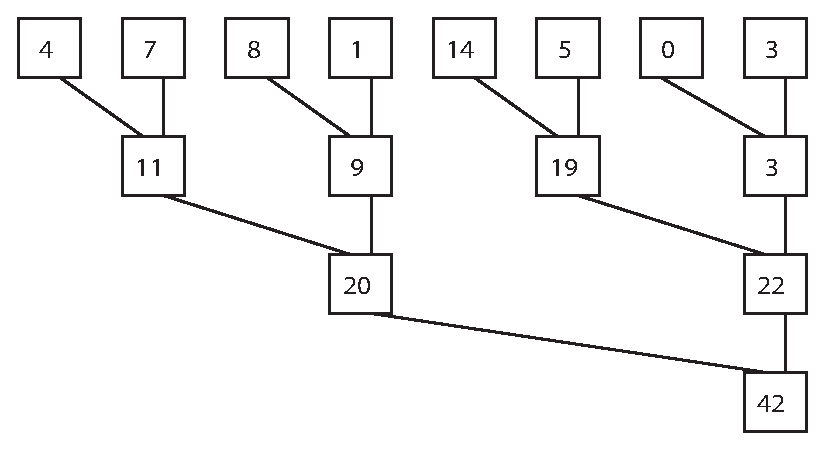
\includegraphics{parallel-left-fold-tree.pdf}
\caption{An illustration of the successive reduction of
  parallel-left-fold where $\oplus$ is set to be addition.}
\label{plfd}
\end{figure}
\vspace{1pc}

Figure \ref{plfd} depicts the operation of \procedure{parallel-left-fold} with each box representing a value that is computed during the operation. Each row of the figure represents a reduction of the original input sequence. The lines entering each box indicate which values contributed to the contained value, and the column that a box appears in indicates the position in memory that is used to store that value. Each column in the figure represents a slot in an array, so boxes that appear in a column with elements below them represent an overwrite to an occupied slot in the array. The final (lowest) element in the $i$th column represents the final value that is stored in the $i$th slot of the array.

An explicit procedure to determine which processor performs each $\oplus$ operation must be devised to complete our implementation of \procedure{parallel-left-fold}. Note that the number of values that are stored for the $j$th reduction of the input sequence is $\lceil \frac{n}{2^j}\rceil$. Thus we need $\lceil \frac{n}{2^i} \rceil$ processors to perform the $i$th (starting at 1) reduction of our sequence. Note that there are exactly $\lceil \frac{p}{2^j} \rceil = \lceil \frac{n}{2^{j+1}} \rceil$ numbers $l$ in the range 0 to $p-1$ for which $(l \mod 2^j = 0)$. This means that the modulus operator together with a variable that is multiplied by two in each iteration can be used to select which processors will be active. Since all $p$ of our processors must be active in the first round, we will initialize this variable to the value of 1. Note that this value also corresponds to the distance between the values that each processor will add in any particular reduction. The pseudo-code labeled Algorithm \ref{plf} describes the rest of the details of our implementation of parallel-left-fold.


\begin{algorithm}[h!]
\label{plf}
\caption{parallel-left-fold where $p = n/2$ and $n=2^k$}
\begin{algorithmic}
\STATE values[pid] $\leftarrow$ input[$2\cdot \mbox{pid}$] $\oplus$ input[$2\cdot \mbox{pid} +1$]
\STATE stride $\leftarrow$ 1
\WHILE{$\mbox{pid} \mod \frac{n}{\mbox{stride}} = 0$ and $\mbox{stride} < n$}
\STATE values[pid] $\leftarrow$ values[pid] $\oplus$ values[pid $+$ stride] 
\STATE stride $\leftarrow$ stride$\cdot 2$
\ENDWHILE
\RETURN values[0]
\end{algorithmic}
\end{algorithm}

\pagebreak

In computing \procedure{parallel-left-fold} in the manner described above, some of the partial sums that constitute the output of \procedure{parallel-prefix-sums} are computed.

\begin{figure}[h!]
\begin{center}
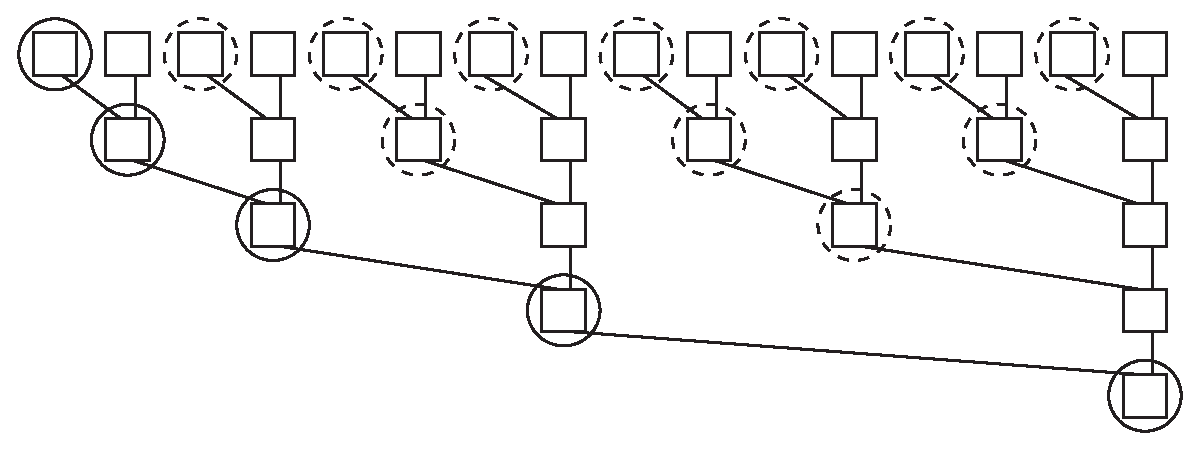
\includegraphics[scale = .75]{correctsums.pdf}
\end{center}
\caption{Each box in the figure that represents the final value in a slot of the temporary array is circled. A solid circle indicates that the value is complete, while a dashed circle indicates that the value is incomplete.}
\label{nonumtree}
\end{figure}

Specifically, all the partial sums that are placed at output indices $2^a-1$ for non-negative integers $a$ are correct. The other sums that are computed as intermediaries to the final sum are incomplete in the sense that they are only correct prefix sums for some continuous subsequence of the input sequence.

In general, the sum in the temporary array at the $i$th index after the execution of parallel-left fold is the sum of the subsequence ending at $a_i$, and including $2^j$ terms\footnote{$a_{i-(2^j-1)},  a_{i-(2^j-1)+1}, \ldots a_i$}, where $j$ is the final round in which that value was modified.

\begin{proof}
What we will prove is that the value at any array index $i$ that is active during the $j$th reduction is the subsequence of length $2^j$ ending at the $i$th value of the input sequence. This directly implies that the value that remains after the execution of the entire algorithm will be the value after the final reduction in which that value was changed.

We prove this claim by induction on $j$. When $j=0$ the values in the temporary array are just the values of the input sequence. Since $j=0$, $2^j = 1$, and indeed, the values of the input sequence are the trivial sums of length one.

Suppose that the node $i$  is active during the $j+1$th reduction step. Then by our induction assumption, its value just before that reduction step is executed is the correct subsequence of length $2^j$. Similarly, the array value that is to be added to our value was also active at the $j$th reduction\footnote{The value at the $z$th array index is active in the $j+1$th round when $z+1 \mod 2^{j+1} = 0$ (and $z \neq 0$). Thus $z - 2^j +  1 = 0 \mod 2^j$, since both $z+1$ and $2^j = 0 \mod 2^j$. This is the index of the value on the left hand side of the $\oplus$ operation.}, and so its subsequence is the $\oplus$ of the sequence of length $2^j$ ending at that index. As noted in the previous section, the distance between terms added in the $j$th reduction is always $2^j$, which means that these two sequences have no overlapping terms, and no missing terms in between them. By the associativity of the operator that is being used, the value that results from applying $\oplus$ to these two terms is value of the subsequence ending at the rightmost index of length $2^j + 2^j = 2 \cdot 2^j = 2^{j+1}$.
\end{proof}

With this fact in hand, it is easy to determine which array indices contain correct values. Since the value at the $i$th index of the array is correct when it contains the $\oplus$ of the $i$ terms, any index $i$ for which $i+1 = \max \{ 2^a : i+1 \mod 2^a = 0 \}$ will contain a correct value. This condition is satisfied when $i+1 = 2^a$ for some $a$.
\vspace{1pc}

One way to fix the incomplete sums issue is to make use of the processors that are inactive in each stage of the algorithm. The suggested algorithm is depicted in figure \ref{fig:naivesums}, and pseudo code is provided in Algorithm \ref{alg:naivepsums}.

\begin{figure}[h!]
\begin{center}
\includegraphics{naivepsums.pdf}
\end{center}
\caption{Each processor is assigned a value in the array. Every processor is active until the stride makes it so that the destination is not a valid entry in the array.}
\label{fig:naivesums}
\end{figure}
\vspace{1pc}

\begin{algorithm}[h!]
\caption{A naive prefix sums algorithm}
\label{alg:naivepsums}
\begin{algorithmic}
\STATE copy input array into array called \var{values}
\STATE $\var{stride} \gets 1$
\WHILE{$\var{stride} < n$}
\IF{$\var{pid} - \var{stride} > 0$}
\STATE $\var{values[pid]} \gets \var{values[pid - stride]} \oplus \var{values[pid]} $
\STATE $\var{stride} \gets \var{stride}\cdot 2$
\ENDIF
\STATE Synchronize Processors.
\ENDWHILE
\end{algorithmic}
\end{algorithm}

Though this figure closely resembles the \procedure{parallel-left-fold} figure, there are some key differences between this algorithm and the \procedure{parallel-left-fold}. First of all, items are no longer ``paired'' so that each element figures in only one sum per round. This means this algorithm requires that the computing system it is running on supports concurrent reads. It also means that twice as many processors are required in the first round of the operation.

The biggest problem with this algorithm is that it is not work-efficient. At least half of the $n$ available processors are active at each level of the algorithm, since the largest stride will be $n/2$. The number levels required to complete the prefix sum operation is $\log n$. This means that $\frac{n}{2}\cdot\log n$ is a lower bound for the number of operations performed by this algorithm. $\frac{n}{2}\cdot \log n \in \mathcal{O}(\log n \cdot n)$, which means that this algorithm requires many more operations than the sequential prefix sums algorithm.

\subsection{Work Efficient Parallel-Prefix-Sum}

The astute reader may have noticed that the structure depicted in figure \ref{nonumtree} is a balanced binary tree. This fact will be essential to the presentation of the work-efficient \procedure{parallel-prefix-sum} algorithm. We introduce some terminology that relates to the tree structure in this diagram.

\begin{itemize}

\item The term ``leaf'' refers to a vertex that has no children. In this case, the leafs of our tree represent the input values to the parallel-left-fold algorithm

\item Note that each non-leaf vertex receives a contribution from two other vertices in our tree. Such a vertex is a ``parent'' of the vertices that are used to compute its value. The left contributor is the ``left-child'' of this vertex, and the right contributor is the ``right-child'' of this vertex.

\item The tree structure that is depicted in figure \ref{nonumtree} is never explicitly represented in memory. Each vertex is associated with an index in the array that is used to store its values. The ``array-index'' of a right-child is the array-index of its parent, while the array index of a left-child in the $j$th level occurs $2^j$ slots before the index of it's parent. The reader should note that there is not a one to one correspondence between array indices and vertices of the tree.

\item The preorder traversal of a tree is a depth-first, left-most walk of its nodes. A vertex $x$ precedes another vertex $y$ if $x$ is reached before $y$ in the preorder traversal of the tree in which they reside.

\item The right-child of a vertex is preceded by its parent, anything that precedes its parent and all of the vertices in the subtree rooted at its parents left-child. A left-child immediately follows its parent in the preorder traversal. That is to say that it is preceded by its parent and anything that precedes its parent.

\item In the parallel-left-fold operation, the value found at each vertex is the sum of the values of the leafs in the subtree rooted at that vertex. 

\end{itemize}

The parallel-prefix-sum algorithm begins with the execution of the parallel-left-fold algorithm exactly as it was presented in the previous subsection. We call this phase of the algorithm the leaf-to-root sweep because it starts at the leaves of the binary tree and ends at the root vertex. The second phase of the parallel-prefix-sums algorithm is a second pass through this binary tree, where each vertex is assigned a new value. This time, we traverse the levels of the binary tree starting at its root root and ending at its  leaves, and thus we call this operation a root-to-leaf sweep. Before the root-to-leaf sweep is executed, the value at the array index of the root vertex, which will always be the final location in the array, is set to be the identity element of our associative operation. The values at all the other locations in the array remain as they are after the leaf-to-root sweep.

In the root-to-leaf sweep, we add the value at the left child of our vertex to the value at the current vertex to produce the value for the right child of the current vertex, and we set the value at the left child to be the value at the current vertex. As mentioned earlier, the array index of the right-child of every vertex in the tree is the same as the index of its parent, so an update of the right-child's array index will overwrite the value of the current vertex. Since we need to set the value at left-child to be the value at the parent node, we must take care to store the value at the current vertex in a temporary variable before we perform the update of the array index of the right-child.

Though it may not yet be clear to the reader, the root-to-leaf sweep operation places the sum of the first $i$ terms of the input sequence in the $i$th slot of the array where it stores values. That is, the values in the array will be the values of the prefix sum operation shifted one to the right, with the identity element in in the $0$th slot of the array. We will now present a proof of this fact:

\setlength{\parindent}{0cm}
\begin{proof}
First, we note that the final iteration of the root-to-leaf sweep occurs at the leaf vertices of our binary tree. Since every array index is associated with some leaf vertex, the final value at each array-index is the value associated with some leaf vertex. The leaf vertex that is associated with the $i$th array index is preceded by every leaf-vertex that is associated with array indices smaller than $i$, but no array indices larger than $i$. That means that the value at a leaf-vertex is the desired value if it contains the sum of the original values of the leaf vertices that precede it. To demonstrate the correctness of our algorithm, we show that this is the case at any vertex after it has been reached by the root-to-leaf sweep.

\vspace{1pc}

\textbf{Claim:} Every vertex will be given the value that is the $\oplus$ of the leaves that precede it during the root-to-leaf sweep.
\vspace{.5pc}
We will demonstrate our claim by induction on the levels of our binary tree.
\vspace{.5pc}

\textbf{Base Case:} 

Our base case occurs at the root level of the tree, where the root node is the only vertex. The root is the first vertex that appears in the preorder traversal, so it is not preceded by any vertices. The value at the array index of the root is correctly set to be the identity element at the beginning of the root-to-leaf sweep.
\vspace{.5pc}

\textbf{Induction Step:}
We seek to show that a vertex at some level in the tree will be given the correct value. We know that this vertex is not the root, and thus it must have a parent that has already been reached by the root-to-leaf sweep. By our induction assumption, the value at the parent is correct.

\vspace{.5pc}
\textbf{Case 1:} The vertex is a left-child.

The only vertex that precedes a left-child that does not precede its parent is the parent itself. Since the parent can't be a leaf, the left-child is preceded by exactly those leaves that precede its parent. Since the left-child receives a copy of its parents value, its value is correct after the root-to-leaf sweep.

\vspace{.5pc}

\textbf{Case 2:} The vertex is a right-child.

The leaves that precede a right-child can be divided into two groups, those that precede its parent, and those that are in the subtree rooted at the left-child of its parent. Earlier, we demonstrated that the upsweep value that resides at the left-child's array index is the $\oplus$ of all the values in its subtree. Thus the $\oplus$ of the value of the parent of the vertex and the value of the left child of the parent of the vertex is the $\oplus$ of all the leaves that precede the vertex.
\end{proof}

\setlength{\parindent}{.5cm}

The pseudo-code labeled Algorithm \ref{epsums} provides an implementation of \procedure{parallel-prefix-sums} that follows the outline we have described in this section. Though it will not play a role in the analysis of the algorithm, the reader should study it closely, as it will serve as the basis of the OpenCL implementation presented later in this section.

\begin{algorithm}[h!]
\caption{parallel-prefix-sums where $p = n/2$ and $n=2^k$}
\label{epsums}
Processors are numbered $1$ to $p$

\procedure{parallel-prefix-sum(input)}:
\begin{algorithmic}[1]
\STATE Copy two values (at $2 \cdot (\var{pid}-1)$ and $2 \cdot (\var{pid}-1) +1)$  from the input array into a temporary array called \var{values}.
\STATE $\var{stride} \gets 1$
\STATE $\var{elm} \gets 2 \cdot \var{pid}$
\WHILE{$\var{stride} < n$}
\IF{$\var{elm} \mod \frac{n}{\var{stride}} = 0$}
\STATE $\var{values[elm-1]}$$\gets$$\var{values[elm-1-stride]} \oplus \var{values[elm-1]}$
\ENDIF
\STATE $\var{stride} \gets \frac{\var{stride}}{2}$
\STATE Synchronize Processors.
\ENDWHILE
\STATE $\var{stride} \gets \frac{n}{2}$
\WHILE{$ \var{stride} > 0$}
\IF{$\var{elm} \mod \var{stride} = 0$}
\STATE $\var{temp} \gets \var{values[elm-1]}$
\STATE $\var{values[elm-1]} \gets \var{values[elm-1]} + \var{values[elm-1-stride]}$
\STATE $\var{values[elm-1-stride]} \gets \var{temp}$
\ENDIF
\STATE $\var{stride} \gets \frac{\var{stride}}{2}$
\STATE Synchronize Processors.
\ENDWHILE
\end{algorithmic}
\end{algorithm}

\subsection{Performance Analysis and Generalization}

Now that we have demonstrated the correctness of our prefix-sum algorithm, we turn our attention to the analysis of its performance. Again, we employ to the tree structured that we have used to represent the operation of the algorithm. We know that our tree is balanced and binary, and that it has $n$ leaves. Thus, the number vertices that are parents of the leaves of the tree will be exactly $\frac{n}{2}$. In general, there will be $\frac{n}{2^j}$ vertices at a depth $j$ away from the leaves of the tree. We want to know how many levels are in the tree, so we solve $\frac{n}{2^j} = 1$, since the level at which there is one node will be the final level of the tree. We find that the number of levels in the tree is $j = \log_2 n$. That means that the runtime of each pass through the tree is $log_2 n$, assuming that the values at each level of the tree can be computed concurrently.

Since there is a one to one correspondence between the vertices in the tree and the operations performed by each a root-to-leaf sweep of the tree, the total the number of leaves in the tree will be the total number of operations performed. We find the number of vertices in a balanced binary with $n$ leaves by summing the number of vertices at each level. We get

$$
1 + 2 + 4 + \cdots + \frac{n}{2} + n = 2n -1
$$

For a leaf-to-root sweep, no operations are performed for the leaf vertices in the tree, so the total work performed is $n$. The total work performed by the \procedure{parallel-prefix-sum} algorithm is the sum of the work done in each kind of sweep or $3n$. $3n \in \mathcal{O}(n)$, so we see that this parallel algorithm is asymptotically work-optimal.
\vspace{1pc}

The \procedure{parallel-prefix-sum} algorithm can easily be generalized so that any number of processors can be used with an input sequence of arbitrary length. No real modifications are needed to support sequence lengths that are not powers of two; this assumption was made to simplify the computation of runtimes, and to ensure that all the vertices of the diagram would be in a single tree. To modify the algorithm so that any number of processors can be used, we introduce processor local phases before and after the parallel phase of the algorithm. Before the parallel phase of the algorithm, each processor sums a section of size $\frac{n}{p}$ to generate a single element that will be used in the parallel operation. The $i$th processor will then use the $i$th element of the prefix sum as an offset value and simply apply the sequential version of the prefix sum algorithm.


%%figure illustrating generalization

\subsection{An Aside}

It would be remiss of the author to fail to address the fact that the naive parallel-prefix-sum algorithm presented earlier has the same parallel runtime as the work-efficient algorithm that was advocated in this section. This assumes, of course, that each level of the \procedure{parallel-left-fold} tree can be computed in parallel in a constant amount of time. This assumption only holds when there are as many processors as there are elements in the input sequence, which is an extremely limiting assumption, even on the massively parallel architecture of the GPU.

Even if we put this issue aside, it is tempting to argue that the work-efficient version of \procedure{parallel-prefix-sum} offers no real benefits over the naive version on GPU hardware. The argument would go something like this:

\vspace{.5pc}

Though fewer instructions will be performed by the work-efficient version of the algorithm, most of the ``saved'' clock cycles are wasted because instructions are executed at the level of the thread warp. Perhaps more explicitly, when the stride of the algorithm is 32 or higher(the assumed size of a thread warp), only one of the work-items in each thread warp will actually be computing something. If the work-item does its job in $c$ cycles, the actual cost of performing that operation is actually $32 \cdot c$.
\vspace{.5pc}

The glaring problem with this argument is that it ignores the fact that memory access is by far the most expensive operation on the GPU. The work-efficient version of \procedure{parallel-prefix-sum} is certain to run much faster than the naive version of the algorithm not because it performs fewer floating point operations, but because it makes fewer requests to local and global GPU memory.

This is not to say that issue that is highlighted in this argument should be ignored. Thread divergence within a thread warp can have drastic effects on the performance of a kernel, and it should be minimized at all costs. Thankfully, we can massage the details of the efficient \procedure{parallel-prefix-sums} algorithm so that drastic thread-divergence of this kind does not occur.

We accomplish this by changing the way processors are selected to be active in each round. Instead of selecting the $2^j$ processors whose process id's have a residue of 0 modulo $2^j$, we simply select the first $2^j$ (or $\frac{n}{2^j}$ in the case of an upsweep) processors to be active in the $j$th round. This means that all the inactive processors at each level will be contiguous, and thus there will be instruction divergence in at most one thread warp in each local work-group.

\subsection{OpenCL Implementation}
\label{sec:opclpsums}

The idiosyncrasies of GPU hardware make the implementation of \procedure{parallel-prefix-sums} exactly as it was described in the previous section impossible. This section describes a reformulation of the algorithm that is suited to the platform, as well as some minor adjustments that boost its performance.

The impossibility of synchronization between threads that are not in the same local work-group presents what is perhaps the largest obstacle to the implementation of \procedure{parallel-prefix-sums} in OpenCL. As indicated in the pseudo-code from the previous section (lines 9 and 19), some type of processor synchronization must occur after each level (iteration of the while loop) of the algorithm has been completed. This is an essential feature of the algorithm that cannot be circumvented; the values that are computed in each level depend on the values that were completed in the previous level. If some thread warp were to get ahead of the others, the values it would retrive from memory would be inaccurate, and the correctness of the result of the computation would be compromised.

This means that we can only run \procedure{parallel-prefix-sums} amongst a group of work-items that belong to the same local work-group. The obvious solution to this problem is to place every work-item in the global work-group in a single local-work group. Unfortunately, this solution has a number of undesirable properties. Chief among them is the fact that synchronization between work-items in a local work-group is only possible because all of the work-items of a local work-group execute on a single compute unit. That means that the single local work-group approach will only allow the utilization of one of the compute units of the target GPU. Worse is the fact that there is a hardware level constraint on local work-group size, which is on the order of 1000 work-items on contemporary GPUs. This means that prefix-sums of sequences longer than 2000 data elements can not be computed with this approach.

We present a resolution to this problem that avoids these issues with a procedure that takes inspiration from the generalization of  \procedure{parallel-prefix-sums} to run on any number of processors. The suggested algorithm is roughly as follows:

\begin{itemize}

\item Determine the largest supported local work-group size, $k$.

\item Divide the input sequence into segments of length $2\cdot k$ (no division in memory is implied here; this is an abstraction), and enqueue a local work-group of size $k$ to compute the local prefix sums of each segment.

\item As it computes the local prefix-sums (just before the final element is cleared for the root-to-leaf phase), a work-item from each local work-group stores the total sum of its segment in an array that has one slot for each local work-group. If the input sequence was of length $n$, then this array would have size $\frac{n}{2k}$. The $i$th work group inserts the sum of the $i$th segment into the $i$th array slot. We will refer to this array as the partial sums array.

\item Check to see if the partial sums array is larger than $k$. If it is, recursively execute the procedure that is being described on that array. If it isn't then calculate the prefix-sums of the array using a single local work-group.

\item Assuming the correctness of this algorithm, the results from the previous step will be the prefix-sums of the partial sums array. That is, the $i$the slot of the resulting array will contain the sum of the all of the elements up to, but not including the $i$th element in the partial sums array. Since the sum of each segment numbered lower than $i$ is represented in some slot of the partial sums array, this value will be the sum of all the elements appearing before the $i$th segment.

\item Each element in the output array currently contains the sum of all the elements preceding it that are contained in the $i$th segment. Thus if we add the sum of all the elements preceding it that are not contained in the $i$th segment, we will get the sum of all the elements that precede it as desired. We do this to each element in a $2k$ segment with an operation called \procedure{UniformAdd}.

\end{itemize}

This description, lengthy though it is, should be regarded as a draft of our open OpenCL algorithm, as some of the important details of the procedure have been glossed over or even completely ignored. In particular, we have defined the algorithm as an single indivisible procedure, though it actually consists of a series of discrete parts, and we have neglected to describe the orchestrating role played by the CPU in its execution.

An explicit prose description of the algorithm would be intolerably inefficient in conveying this missing information, so we have provided pseudo-code descriptions of each of the various phases of the algorithm  instead. Each pseudo-code will be followed by analysis of the important details it contains, but the reader is encouraged to fully absorb the content of each of these figures before continuing.

\begin{algorithm}[h!]
\caption{The Prefix Sums CPU Host Program}
\label{alg:psumshost}
\begin{algorithmic}[1]
\STATE $\var{g_size} \gets $ the maximum work group size.
\STATE $\var{elem_count} \gets $ the size of the input sequence.
\STATE $\var{temp} \gets \var{elem_count}$
\WHILE{$\var{elem_count} > 1$}
\STATE Allocate an array of the size $\var{temp}$ in the global memory of the device.
\STATE Store a handle to this array in a slot of an array for storing these references called $\var{p_sums_mem}$
\STATE $\var{temp} \gets \lceil\max \{1, \frac{\var{temp}}{2\var{g_size}}\} \rceil$
\ENDWHILE
\STATE Copy the values of the input sequence into the first array of \var{p_sums_mem}.
\STATE $\var{prefix_sums(p_sums_mem, 0, elem_count, g_size)}$
\end{algorithmic}
\vspace{1pc}


\procedure{prefix_sums(p_sums_mem, level, elem_count, g_size)}
\begin{algorithmic}[1]
\STATE $\var{num_work_elems} \gets $ the largest multiple of $2\cdot \var{g_size}$ that is smaller than $\var{elem_count}$.
\STATE $\var{remaining_elems} = \var{elem_count} - \var{num_work_elems}$
\STATE $\var{next_count} \gets \frac{\var{num_work_elems}}{2\cdot \var{g_size}}$, add 1 if $\var{remaining_elems} > 0$
\IF{$\var{next_count} > 1$}
\STATE $\var{store_segment_sums} =$ True
\ENDIF
\IF{$\var{num_work_elems} > 0$}
\STATE execute \procedure{segment_sums(p_sums_mem[level], p_sums_mem[level+1], 0,store_segment_sums)} with a global work-group of size $\frac{\var{num_work_elems}}{2}$ and local work-groups of size \var{g_size}.
\ENDIF
\IF{$\var{remaining_elems} > 0$}
\STATE execute \var{segment_sums(p_sums_mem[level], p_sums_mem[level$+1$], $2 \cdot$ num_work_items, store_segment_sums)}
with a global work-group size of $ \lceil \var{remaining_elems} \rceil$ and local work-groups of size $ \lceil \var{remaining_elems} \rceil$
\ENDIF
\STATE Wait for both kernel tasks to finish.
\IF{$\var{store_segment_sums}$}
\STATE \var{prefix_sums(psums_mem, level$ + 1$, next_count, g_size)}
\STATE execute \var{uniform_add(psums_mem[level], psums_mem[level$+1$])} with a global work-group of size $\frac{\var{num_work_elems}}{2}$ and local work-groups of size $\var{g_size}$ with a global work-group size of $ \lceil \var{remaining_elems} \rceil$ and local work-groups of size $ \lceil \var{remaining_elems} \rceil$
\STATE
\ENDIF
\end{algorithmic}
\end{algorithm}



The following while loop will allocate all of the partial sums arrays that will be needed in the recursive calls to compute segment prefix sums. References to each of these memory objects will be stored in an array

\chapter{GPU Graph Algorithms}

\section{Modified Matrix Multiplication}

This section presents an algorithm that solves the all-pairs shortest paths problem by using a modified form of matrix multiplication.

\section{Algorithm Description}

The complete structure of a graph on $|V|$ vertices can be represented with a $|V| \times |V|$ matrix. Such a matrix is called an adjacency matrix. In the construction of a graph's adjacency matrix, the vertices are enumerated with the natural numbers in the range $1$ to $|V|$. The $i,j$th entry of the matrix is set to be 1 if $(i,j) \in E$, and is set to be 0 if $(i,j) \not \in E$.

The concept of an adjacency matrix can be reformulated to represent the structure of a weighted graph. In a weighted adjacency matrix, the $(i,j)$th entry is set to be the weight of $(i,j)$ if $(i,j) \in E$ and $\infty$ otherwise. Using notation that was introduced in previous chapters\footnote{See section \ref{sec:bf} for a description of the function $d_{i,j}$ and \ref{ch:mm} for the details of the notation $A_{i,j}$}:
\begin{equation}
\label{eq:ajmdef}
A_{i,j} = d_{i,j}(1)
\end{equation}
In section \ref{ch:mm}, the matrix multiplication operation was defined in terms of the operators $\oplus$ and $\otimes$. The pseudo-code provided in that section described algorithms to perform the most typical kind of matrix multiplication, where $\oplus$ is taken to be conventional addition and $\otimes$ conventional multiplication, but the techniques they describe can be adjusted to any form of matrix multiplication where $\oplus$ and $\otimes$ are associative operations.

When $\oplus$ is taken to be the operation of minimization, and $\otimes$ the operation of addition, the matrix product of an adjacency matrix with itself takes on special significance. To see why, we write out the value of the $i,j$th entry of the product $A \cdot A$, and apply equation \ref{eq:ajmdef} and our choices of $\oplus$ and $\otimes$:
\begin{equation}
\begin{array}{c}
(A \cdot A)_{i,j} = (A_{i,1} \otimes A_{1,j}) \oplus (A_{i,2} \otimes A_{2,j}) \oplus \cdots \oplus (A_{i,|V|} \otimes A_{1,|V|}) = \\
\label{eq:mmadid}
(d_{i,1}(1) + d_{1,j}(1)) \min (d_{i,2}(1) + d_{2,j}(1)) \min \cdots \min (d_{i,|V|}(1) + d_{1,|V|}(1))
\end{array}
\end{equation}
The binary minimum operation applied to a sequence of values is simply the minimum of the sequence. Thus we can re-write equation \ref{eq:mmadid} as:
\begin{equation}
\begin{array}{c}
\label{eq:fmmid}
\min \{ (d_{i,1}(1) + d_{1,j}(1)), (d_{i,2}(1) + d_{2,j}(1)),\ldots, (d_{i,|V|}(1) + d_{1,|V|}(1)) \}  \\
= \min \{d_{i,n}(1) + d_{n,j}(1) : n \in V \} = (A \cdot A)_{i,j} 
\end{array}
\end{equation}
The reader is forgiven if they do not recall equation \ref{eq:did}, and so it is reprinted here:
$$
d_{u,v}(n+1) = \min \{d_{u,w}(n) + f((w,v)) : w \in V, \, (w,v) \in E \} \cup \{d_{u,v}(n)\}
$$
Note that 
\begin{displaymath}
   d_{n,j}(1) = \left\{
     \begin{array}{lcl}
       0 & : &n = j \\
       f((n,j)) & : &(n,j) \in E \\
       \infty & : &n \neq j, (n,j) \not \in E \\
     \end{array}
   \right.
\end{displaymath}
This means that:
$$
\{d_{i,n}(n) + d_{n,j}(1) : n \in V \} =
$$
$$
\min \{d_{u,w}(n) + f((w,v)) : w \in V, \, (w,v) \in E \} \cup \{d_{u,v}(n)\} \cup \{d_{u,w}(n) + \infty :  (w,v) \not \in E\}
$$
Clearly, the last set in this union can't affect the minimum of the union, thus we have:
\begin{equation}
\label{yes}
\min\{d_{i,n}(n) + d_{n,j}(1) : n \in V \} = d_{i,j}(n+1)
\end{equation}
Returning to equation \ref{eq:fmmid}:
$$
(A \cdot A)_{i,j} = d_{i,j}(2)
$$
That is, the $i,j$th entry of the product $(A \cdot A)$ is the weight of the shortest path of length 2 from $i$ to $j$.
This fact can be generalized by induction on the number of multiplies of $A$. Let $A^n$ be $A$ multiplied by itself $n$ times. Our claim is as follows:
\begin{equation}
(A^n)_{i,j} = d_{i,j}(n)
\end{equation}
\begin{proof}
We have already demonstrated the base case.
\vspace{.5pc}

\textbf{Induction Step}
We assume that $(A^k)_{i,j} = d_{i,j}(k)$.

Then $((A^k)\cdot A)_{i,j} = \min \{d_{i,n}(k) + d_{n,j}(1) : n \in V \}$, and by equation \ref{yes},

$$
((A^k)\cdot A)_{i,j} = (A^{k+1})_{i,j} = d_{i,j}(k+1)
$$
\end{proof}

We have demonstrated  that $n$ modified matrix multiplications of the weighted adjacency \label{alg:pbf}matrix of a graph yields the weight of the shortest $n$-edge paths for every pair of paths in the graph. Given that shortest paths can contain no more than $|V|-1$ edges, the execution of $|V| - 1$ such multiplies calculates the shortest path weights of any graph. The kernel that performs the modified matrix multiplication of this algorithm is not appreciable different to the kernel that performs conventional matrix multiplication from section \ref{ch:mm}. As such no pseudo-code for this kernel will be presented. However, there are several interesting details of the OpenCL implementation of the algorithm that the author wishes to present.
\vspace{1pc}

\subsection{A Performance Optimization}
The natural algorithm for performing the calculation of $A^n$ from $A$ involves applying the matrix multiplication algorithm $n-1$ times; $A^2$ is calculated by multiplying $A$ by itself, $A^3$ is calculated by multiplying $A^2$ by $A$ and this pattern continues until we have calculated $A^{n}$. Because $\oplus$ and $\otimes$ are assumed to be associative operators, any type of matrix multiplication is itself associative. Because of this fact, the following identity holds:

\begin{displaymath}
   A^n = \left\{
     \begin{array}{lcl}
       A^{n/2} \cdot A^{n/2} & : & n \mbox{ is even} \\
       A^{n/2} \cdot A^{n/2} \cdot A  & : & n \mbox{ is odd}\\
     \end{array}
   \right.
\end{displaymath}

This equation enables a performance optimization in the calculation of the matrix $A^{n}$ from $A$. We view the above equation as a recurrence, and calculate $A^n$ in the following way:

\begin{algorithm}
\procedure{matrixExponent(matrix, exponent)}
\begin{algorithmic}[1]
\IF{$\var{exponent} > 3$}
\STATE $\var{half} \gets \var{matrixExponent(matrix, exponent/2)}$
\STATE $\var{res} \gets \var{multiply(half, half)}$
\ELSE
\STATE $\var{res} \gets \var{multiply(matrix, matrix)}$
\ENDIF
\IF{$\var{exponent} \mod 2 = 1$}
\STATE $\var{res} \gets \var{multiply(res, matrix)}$
\ENDIF
\RETURN \var{res}
\end{algorithmic}
\end{algorithm}

An even simpler procedure can be used to calculate shortest paths weights using modified matrix multiplication. This is because shortest paths weights are contained in any matrix $A^n$ where $n > |V|-1$. That is, we are not specifically interested in the matrix $A^{|V| - 1}$, but any matrix that is large enough. This allows us to ignore the separate case when $n$ is odd, and simply calculate the matrices $A^{2^k}$ until $2^k$ is larger than $|V| - 1$.

\subsection{Calculating Paths}

Thus far, the algorithm we have described merely calculates the weight of the shortest path between every pair of vertices. It is often important to calculate the sequence of vertices that provides this shortest path weight. We present a small modification to our algorithm that allows these sequences to be calculated.

The basic idea of this modification is to maintain a separate $|V| \times |V|$ matrix of predecessor values whose $i,j$th entry is the penultimate vertex in the shortest path between $i$ and $j$. It is clear how the matrix should be initialized: the $i,j$the entry of the predecessor matrix will be $i$ if there is an edge between $i$ and $j$ and $\infty$ otherwise.

This matrix is updated in accordance with any updates to the path weight matrix. That is, when the $i,j$the entry of the path weight matrix is updated to be the weight of the path from $i$ to $m$ plus the weight of the path from $m$ to $j$, the value at the $m,j$th entry of the predecessor matrix is copied into its $i,j$th entry. 

The shortest path from $i$ to $j$ is retrieved from the finalized predecessor matrix with the following procedure:

\begin{itemize}

\item Start at the $i,j$th entry of the matrix, and add $j$ to the end of the path.

\item If the value at this entry is $\infty$, there is no path between $i$ and $j$.

\item If the value at this entry is $m$, place it before the other entries in this path.

\item Now go to the $i,m$th entry of the matrix

\item Repeat this procedure until the $i,i$the entry of the matrix is reached.

\end{itemize} 

\subsection{Detecting Negative Cycles}

One of the advantages of the APSP matrix multiplication procedure is that it supports graphs with negative weight edges. As mentioned section \ref{sec:bf}, when a negative weight graph contains a cycle of negative weight, some shortest paths in the graph are undefined. Nonetheless, if we perform APSPMM on a graph with a negative weight cycle, a shortest path weight will appear in every entry of the matrix. That is, the algorithm will return shortest paths weights even for pairs of vertices between which there is no shortest path. In some situations this could be undesirable behavior. Thankfully, it is possible to detect negative weight cycles with the APSP matrix multiplication with no modifications.

Consider that a cycle is a path that starts and ends at the same place and that we initialize the $i,i$the entries of the path weight matrix to be the value 0. These facts imply that if there is a cycle of negative weight that contains $i$, the $i,i$th entry of the path weight matrix will contain a negative value. Thus we can detect any negative weight cycles by scanning the diagonal of the shortest path weight matrix for negative values.

The memory of a negative weight cycle in a graph does not necessarily imply that there are no shortest paths in the graph at all. It is possible that some applications of APSP might still have use for the valid shortest paths in a graph with a negative weight cycle. The shortest path value provided by the APSPMM algorithm is invalidated if and only if it passes through a vertex that is part of a negative weight cycle. To test a shortest path for validity, simply check the $i,i$the entry of the shortest path matrix for negative values for each $i$ in the path.

\section{Parallelized Bellman-Ford}

This section describes an OpenCL procedure that solves the SSSP problem on graphs with arbitrary edge weights. It is inspired by the Bellman-Ford algorithm, but it departs from the classical implementation in several important ways. 

\subsection{Algorithm Description}

Recall that the idea behind the Bellman-Ford algorithm is to perform an edge-relax of every edge in the problem graph $|V|-1$ times. In the sequential version of the algorithm, a looping control statement is used to iterate over the edge list of the graph and relax one edge at a time. The correctness of the algorithm doesn't depend on the order in which edges are relaxed; the only requirement is that every edge must be relaxed for the $j$th time before any edge is relaxed for the $j+1$st time. This makes the Bellman-Ford algorithm an excellent candidate for parallelization.

In particular, it is the inner loop of the Bellman-Ford algorithm that is amenable to parallelization. The outer loop must still be performed in sequence, as per the requirement described in the last paragraph. The natural parallelization of Bellman-Ford is as follows.

\begin{algorithm}
On $p = |E|$ processors:
\begin{algorithmic}[1]
\FOR{$0 to |V|-1$}
\STATE \var{edge-relax(edges[id])}
\STATE Synchronize Processors.
\ENDFOR
\end{algorithmic}
\end{algorithm}

Though we may not have $|E|$ processors on a GPU, we can easily port this algorithm into OpenCL, by enqueuing $|E|$ work-items, each of which will run a kernel that relaxes a single edge in the graph. Synchronization is achieved by executing the for loop on line 1 on the host device and executing a \var{clFinish} command between each set of edge-relaxes.

There is a problem with this algorithm, at least as far as its implementation on GPU hardware is concerned. Consider a graph where $a,b,c \in V$ and $(a,b), (c,b) \in E$. In the execution of the aforementioned procedure on such a graph, distinct work-items might simultaneously relax the edges $(a,b)$ and $(c,b)$. Suppose that both work-items determine that the relaxation of their respective edges yields a shorter path to $b$. Both work-items will attempt to update the path-estimate and predecessor values associated with $b$, which are stored in global memory. If the path-lengths yielded by each of these relaxes is not the same, this situation can jeopardize the correctness of the algorithm. There is no way to guarantee that the smaller path update will be the one that is stored by the device, and as such, some shortest paths might go undetected, even after $|V|-1$ sets of edge relaxes. Furthermore, it can not be assumed that the path-weight value that is stored will come from the same edge-relax as the predecessor value that is stored. If the device were to save the smaller path weight, but the predecessor associated with the larger path, the algorithm might produce a path-tree with incorrect weight estimates for some shortest paths.

This example highlights the unique character of the data-parallelism exhibited by the Bellman-Ford algorithm; though both the input and output of each set of edge-relaxes is data parallel, the granularity of the input parallelism is much finer.  The procedure we have described above fails because it parallelizes at the level of input, without providing any means for the resolution of output conflicts.

The solution to this problem is clear: some type of conflict resolution must be provided. Specifically, minimization must be performed over the output of the relaxes ending at each vertex.  One way to do this is to parallelize Bellman-Ford at the level of output. Instead of using a processor for each edge, we use a processor for each vertex. Each processor is responsible for performing all of the edge-relaxes that end at that vertex, and selecting the update value with minimum path weight. The figure labeled Algorithm \ref{alg:pbf} provides a pseudo-code description of this algorithm.

\begin{algorithm}
\caption{A pseudo-code description of Parallelized Bellman Ford.}
\label{alg:pbf}
\begin{algorithmic}[1]
\STATE $\var{vertex} \gets \var{vertices[id]}$
\IF{$\var{vertex}$ is the source}
\STATE $\var{vertex.weight} \gets 0$
\ELSE
\STATE $\var{vertex.weight} \gets \infty$
\ENDIF
\FOR{$\var{edge} \in vertex.edges$}
\STATE $\var{update} = \var{edge.weight} + \var{edge.source.weight}$
\IF{$\var{update} < \var{vertex.weight}$}
\STATE $\var{vertex.weight} \gets \var{update}$
\STATE $\var{vertex.pred} \gets \var{edge.source}$
\ENDIF
\ENDFOR
\end{algorithmic}
\end{algorithm}

This pseudo-code makes extensive use of references (memory address data types), and as such, it is not suitable for implementation in OpenCL. References that are copied from the host device to an OpenCL device are useless; the GPU will interpret such values as addresses in its own memory system, which will not contain the same values as their counterpart addresses on the CPU, unless by chance. To implement this algorithm in OpenCL, we must reformulate it so that it uses simpler data types. The graph representation used by our implementation comprises the following elements:

\begin{itemize}

\item \var{edge_weights} - An array of size $|E|$ that stores the edge weights of each edge.

\item \var{edge_sources} - An array of size $|E|$ that stores the source of each edge.

\item \var{weights} - An array of size $|V|$ that is used to store the path-weights for each vertex.

\item \var{edge_counts} - An array of size $|V|$ that stores the number of incoming edges to each vertex.

\item \var{vertex_edge_index} - An array of size $|V|$ the starting index for edges that end at each vertex.

\end{itemize}

It should be obvious that the $i$th slots of each of the arrays of size $|V|$ contain information about a particular vertex, and the $i$th slots of the arrays of size $|E|$ contain information about a particular edge. It is also assumed that the edge arrays are sorted so that edges ending at the same vertex are contiguous in memory. Before we continue with the presentation of our OpenCL algorithm, we provide a brief description of how this representation can be computed from a weighted edge adjacency list, \var{edges}. We assume that vertices are represented with the numbers $1$ to $|V|$, and edges comprise source, destination and weight member variables.

\begin{itemize}

\item Sort the edge array, using the destination vertex as a key value. It is now easy to make the edge arrays.

\item Fill the array \var{vertex_edge_index}, by iterating through the edge array and adding an entry each time the destination vertex of an edge is not the same as it was before. In pseudo-code:

\begin{algorithmic}
\STATE $\var{count} \gets 0$
\STATE $\var{vertex_Edge_index[0]} \gets 0$
\STATE $\var{vertex} \gets 0$
\WHILE{$\var{count} < |E|$}
\IF{$\var{edges[count].destination} \neq \var{vertex}$}
\STATE $\var{edge_counts[vertex]} \gets \var{count} - \var{vertex_edge_index[vertex]}$
\STATE $\var{vertex} \gets \var{vertex} + 1$
\STATE $\var{vertex_Edge_index[vertex]} \gets \var{count}$
\COMMENT{It is important not to iterate the count here; the current edge does not belong to new vertex if the vertex has no edges.}
\ELSE
\STATE $\var{count} \gets \var{count} + 1$
\ENDIF
\ENDWHILE
\end{algorithmic}
\end{itemize}

A full OpenCL pseudo-code description of Algorithm \ref{alg:pbf} has been omitted, as it would not offer the reader much in the way of new information. However, there are two non-trivial details of the OpenCL implementation, to which the author would like to draw the reader's attention.

As currently implemented, our algorithm requires that each work-item load all of the edge data it will use from global memory itself. In other words, each work-item must perform $2 \cdot k$ individual global memory access requests where $k$ is the number of edges that end at the work-items vertex. The memory efficiency of the algorithm can be improved if work-items cooperate in loading edge data before they begin the performance of their independent edge-relaxes. This is accomplished by a procedure that is similar to the one that was used to improve the matrix multiplication algorithm in section \ref{ch:mm}. Work-items are grouped into local-work groups that are exactly the size of a thread warp. They alternate between a phase where edges are loaded into memory, and a phase where edge-relaxes are performed. The alternating structure of the procedure is necessary because it may be that some vertices have so many incoming edges that their associated data can't fit into local memory. Loading edge data into memory in chunks that are the size of a thread warp provides optimal performance because doing so minimizes work-item divergence.

The performance of Parallel Bellman-Ford is further improved on GPU devices if the vertices of the problem graph are sorted and re-enumerated according to the number of incoming edges they have. This makes it so that work-items in the same thread warp have a number of incoming edges that is as close together as possible. If this re-enumeration is not performed, extreme work-item divergence may result. Consider what happens when a work-item that is assigned some vertex with thousands of incoming edges appears in a thread warp where all the other work-items are assigned vertices that have only a few incoming edges. Since the execution of the thread warp will only terminate after all its work-items have finished their work, thousands of clock cycles will pass where these other work-items have nothing to do.

\section{Input Parallel Bellman-Ford}

The previous section described an approach to the implementation of Parallelized Bellman-Ford where the granularity of the parallel portion of the algorithm was reduced to avoid concurrent writes to the same location in memory. This allowed the processes of minimization and writing to global memory to occur within the \var{edge-relax} procedure, as it does in the sequential version of the algorithm. In this section, we describe an algorithm that performs minimization, edge-relaxation and global memory updates separately in order to avoid sacrificing parallelism. We will refer this algorithm as Input Parallel Bellman-Ford or IPBF, and we will refer to the algorithm of the previous section as Output Parallel Bellman-Ford or OPBF.

\subsection{Algorithm Description}

As hinted in the previous paragraph, the IPBF algorithm comprises three major stages. In the edge-relax stage of the algorithm, every edge in the problem graph is relaxed. The values associated with each edge-relax are written into a temporary array of size $|E|$. As in the OPBF algorithm, we assume that the edges are sorted so that all the edges that end at a particular vertex are contiguous in memory. This allows us to use a modified version of the \procedure{parallel prefix-sum} algorithm of section \ref{sec:opclpsums} that we will refer to as the segment scan to determine which edge-relax gives the shortest path to each vertex. Segmented scan is a generalized version of prefix-sums that allows the input sequence to be divided into segments. The $i$th entry of the output array of segment scan is the $\oplus$ the elements occurring at or before the $i$the slot of the input array that are in the same segment as the $i$the element of the input array.

The segmented scan that is performed in IPBF uses binary minimization as its associative operator. A new segment is marked at any point where the edges of each vertex begins. These indices are simply the entries of the \var{vertex_edge_index} array. After the segmented scan is finished, the shortest path update for each vertex will reside at the final entry that is associated with any segment. These entries can also be found with the entries of the \var{vertex_edge_index} array. The minimum update for the $i$th vertex can be found at the $\var{vertex_edge_index[i+1]} - 1$th index of the output array (assuming that that vertex has any edges at all). The 

To summarize, the IPBF algorithm consists of 3 kernels:

\begin{itemize}

\item The edge-relax kernel performs edge-relaxes of each edge and stores their values in a temporary array. This kernel is executed with $|E|$ work-items.

\item The segment-min kernel performs a segmented scan of these edge-relax values. This kernel is executed with $|E|$ work-items

\item The finalization kernel updates the path-weight and predecessor values of each vertex by checking the appropriate value in the output of the segmented scan kernel. It only performs an update if the minimum relax value is an improvement. This kernel is executed with $|V|$ work items.

\end{itemize}

\subsection{A Possible Refinement}

The relaxation of an edge whose source vertex's path weight was not updated in the last set of edge-relaxations can not possibly cause an update. In light of this fact, it may strike the reader as strange that the Bellman-Ford algorithm relaxes every single edge in the problem graph in every set of edge-relaxes. Indeed, it is not hard to concoct a graph for which the Bellman-Ford algorithm appears to obstinately perform the same edge-relax calculation over and over again with no hope of obtaining a meaningful result.

This subsection describes a version of IPBF that is informed by the observation of the previous paragraph. It introduces additional stages into the IPBF pipeline so that only edges whose source vertices were active in the last set of edge-relaxes are performed.

In this version of the IPBF algorithm, the problem graph's edges are sorted so that contiguous edges share source vertices, rather than destination vertices. This change complicates some aspects of the algorithm, but it also allows edges to be more easily grouped according to whether or not they should be relaxed. The following modifications to IPBF enable the selective scheduling of edge-relaxes:

\begin{itemize}

\item When an update is made to a vertex's values during the finalization phase of the algorithm, a value of 1 is placed in the vertex's index in an array of size $|V|$ to indicate that the update occurred. Otherwise 0 is placed in the vertex's slot.

\item A prefix-sum with $\oplus$ set to be addition, is performed on this array. The $i$th entry of the output of this array will be the number of vertices with index smaller than $i$ that were updated in the most recent set of edge-relaxes. 

\item This means that we can produce a list (contiguous set of array entries) of the vertices that were active in the most recent set of edge-relaxes by placing the $i$th vertex at the index given by the output of the prefix sum array if it was active in last round.

\item Another kernel places the outgoing edge counts of each of these vertices in an array that is indexed in the same way.

\item The prefix sums of the outgoing edge counts array are computed.

\item We enqueue the number of work-items given by the total sum of this array to perform edge-relaxes. The prefix sums outgoing edge counts array are used to determine the vertex that owns each work item.

\end{itemize}


\chapter*{Conclusion}
\addcontentsline{toc}{chapter}{Conclusion}
\chaptermark{Conclusion}
\markboth{Conclusion}{Conclusion}
\setcounter{chapter}{4}
\setcounter{section}{0}

\section{Implementation Results}

The APSP multiplication algorithm and the Output Parallel Bellman-Ford algorithm described in the previous chapter were implemented in OpenCL and tested on graphics hardware. As of the writing of this paper, the implementation of the refined Input Parallel Bellman-Ford is not yet complete. However, many of the kernels of the algorithm's pipeline have been successfully implemented.

The algorithms were tested on a 2011 Apple MacBook Pro with a 2GHz Intel Core i7 processor and 4GB of 133 MHz DDR3 RAM. The graphics processor onboard this device was an AMD 6490M with 256MB of memory.

\subsection{APSP Matrix Multiplication}

The APSP Matrix Multiplication algorithm was tested with randomly generated adjacency matrices. Two different techniques were used to generate these random matrices. The first of these placed a random finite value between 0 and 400 at each entry in an $n \times n$ array, except at entries along the diagonal of the array, which were set to be 0. That is, it created a random adjacency matrix where every vertex is connected by an edge. The second adjacency generation procedure was more complicated. The entries of the array were initialized to be infinity. Then $n/4$ random entries in each row were given a random finite edge weight between 0 and 400. Finally, the entires along the diagonal were set to 0. This technique generates an adjacency matrix that represents a graph where every vertex has exactly $n/4$ edges.

Figure \ref{fig:apspruntime} plots the runtime of the APSP Multiplication algorithm on our testing hardware against the number of vertices in the problem graph. The type of random matrix used seemed to have no effect on the runtime of the algorithm, so we do not distinguish between which type was used in this figure. This fact seems to indicate that the actual structure of the problem graph has no effect on the efficiency of this algorithm.

\begin{figure}[h!]
\begin{center}
\includegraphics[scale = .75]{APSPgraph.pdf}
\end{center}
\caption{A graph of the runtime APSP Matrix Multiplication against the number of vertices.}
\label{fig:apspruntime}
\end{figure}

The reader may wonder why this algorithm was not tested on larger problem sizes. The reason for this is simple; the adjacency matrix of a graph with as few as 4096 vertices contains $4096^2 = 16,777,216$ entries. Each of these entries requires 4 bytes of memory, which means that the total amount of memory necessary to represent the adjacency matrix of a 4096 vertex graph is $67,108,864$ bytes, or about 67MB. At least two blocks of memory of this size are needed --one for input and one for output-- and it is also required that these blocks be contiguous. On a graphics card with 256MB of global memory that must also hold several frame buffers and other graphical data, it is unlikely that two blocks of this size will be available. These massive memory requirements are not a feature of the matrix multiplication algorithm, but an inherent feature of the APSP problem itself, the size of the answer to the APSP problem is exponential in the number of vertices as there are $n^2$ ordered pairs of vertices.

Given the sheer number of values that must be computed in the APSP problem, the large runtimes of this algorithm even for problem sizes smaller than 5000 vertices is understandable, if a bit disappointing.

%It takes only a glance at \ref{fig:apspruntime} to see that the runtime of APSP is exponetial in the number of vertices. This result should be expected since the number of values in the output is exponential in the number of vertices in the input. 

\subsection{Output Parallel Bellman-Ford}

The Output Parallel Bellman-Ford algorithm was tested with randomly generated graphs with varying numbers of vertices, and a fixed ratio between the number of edges outgoing from each vertex and the number of vertices. Each vertex was given a fixed number of edges whose destinations and edge weights were chosen randomly.



This problem is particularly severe for graphs that have relatively low connectivity (graphs for which the number of edges involving each vertex is relatively small).
The reader should note that this modification offers no theoretical improvements on the Bellman-Ford algorithm. A scenario where a significant portion of the edges in the problem graph are active in every round is certainly possible. Because it introduces many algorithmic complications, performance gains can only really be realized for very large and very sparse graphs.




\begin{comment}
  \backmatter 

    \bibliographystyle{bsts/mla-good} % there are a variety of styles available; 
    \nocite{*}
    \bibliography{thesis}
\end{comment}
\end{document}
